% -- Anfang Präambel
\documentclass[german,  % Standardmäßig deutsche Eigenarten, englisch -> english
parskip=full,  % Absätze durch Leerzeile trennen
%bibliography=totoc,  % Literatur im Inhaltsverzeichnis (ist unüblich)
%draft,  % TODO: Entwurfsmodus -> entfernen für endgültige Version
]{scrartcl}
\usepackage[utf8]{inputenc}  % Kodierung der Datei
\usepackage[T1]{fontenc}  % Vollen Umfang der Schriftzeichen
\usepackage[ngerman]{babel}  % Sprache auf Deutsch (neue Rechtschreibung)

% Mathematik und Größen
\usepackage{amsmath}
\usepackage{amssymb} %Mathematische Symbole, aufrufbar mit mathbb{}
\usepackage[locale=DE,  % deutsche Eigenarten, englisch -> US
separate-uncertainty,  % Unsicherheiten seperat angeben (mit ±)
]{siunitx}
\usepackage{physics}  % Erstellung von Gleichungen vereinfachen
\usepackage{yfonts}  % Frakturschrift für Real- und Imaginärteil komplexer Größen

\usepackage{graphicx}  % Bilder einbinden \includegraphics{Pfad/zur/Datei(ohne Dateiendung)}

% Gestaltung
%\usepackage{microtype}  % Mikrotypographie (kann man am Ende verwenden)
\usepackage{booktabs}  % schönere Tabellen
%\usepackage[toc]{multitoc}  % mehrspaltiges Inhaltsverzeichnis
\usepackage{csquotes}  % Anführungszeichen mit \enquote
\usepackage{caption}  % Anpassung der Bildunterschriften, Tabellenüberschriften
\usepackage{subcaption}  % Unterabbildungen, Untertabellen, …
\usepackage{enumitem}  % Listen anpassen
\setlist{itemsep=-10pt}  % Abstände zwischen Listenpunkten verringern

% Manipulation des Seitenstils
\usepackage{scrpage2}
% Kopf-/Fußzeilen setzen
\pagestyle{scrheadings}  % Stil für die Seite setzen
\clearscrheadings  % Stil zurücksetzen, um ihn neu zu definieren
\automark{section}  % Abschnittsnamen als Seitenbeschriftung verwenden
\ofoot{\pagemark}  % Seitenzahl außen in Fußzeile
\ihead{\headmark}  % Seitenbeschriftung mittig in Kopfzeile
\setheadsepline{.5pt}  % Kopzeile durch Linie abtrennen

\usepackage[hidelinks]{hyperref}  % Links und weitere PDF-Features

% TODO: Titel und Autor, … festlegen
\newcommand*{\titel}{Quantenanalogie}
\newcommand*{\autor}{Tom Drechsler, Konstantin Schmid}
\newcommand*{\abk}{QA}
\newcommand*{\betreuer}{Max Mende}
\newcommand*{\messung}{22.11.2019}
\newcommand*{\ort}{REC/D301}

\hypersetup{pdfauthor={\autor}, pdftitle={\titel}}  % PDF-Metadaten setzen
\begin{document}
% automatischen Titel konfigurieren
\titlehead{Fortgeschrittenen-Praktikum \abk \hfill TU Dresden}
\subject{Versuchsprotokoll}
\title{\titel}
\author{\autor}
\date{\begin{tabular}{ll}
Protokoll: & \today \\
Messung:  & \messung \\
Ort: & \ort \\
Betreuer:  & \betreuer
\end{tabular}}

% -- Ende Präambel


\begin{titlepage}
\maketitle  % Titel setzen
\tableofcontents  % Inhaltsverzeichnis
\end{titlepage}

% Text Anfang
\section{Versuchsziel und Überblick}
Ziel des Versuchs ist es Quantenphysik einfach zu erklären und anschaulich zu interpretieren. Grundlage dafür bietet die Überlegung, dass Elektronen Materiewellen sind und bei diesen somit auch die Phänomene Reflexion, Beugung, Brechung, Überlagerung, Interferenz und stehende Wellen auftreten. Somit sollte es auch möglich sein dies mit Wellen, deren Wellenlängen in einem vergleichsweise makroskopischen Bereich liegen (für z.B Schall einige cm), zu rekonstruieren.
\newline Mit Hilfe eines Lautsprechers sollen Schallwellen erzeugt werden, die in einen Resonator eingesperrt werden. Dieser hat je nach zu betrachtender Analogie eine andere Form, die im jeweiligen Versuchsunterpunkt diskutiert werden wird. Danach wird die Ausbildung stehender Wellen untersucht, da diese unter gleichen Randbedingungen die jeweilige quantenmechanische Lösung gut modellieren. Die gebundenen Lösungen der Schrödinger-Gleichung sind nämlich stehende Wellen.

\section{Theoretische Grundlagen}

\subsection{Quantenmechanisches Teilchen in einer Box}
In diesem Teilversuch wird ein Röhrenresonator verwendet. Dies ist ein geschlossener Hohlzylinder der Länge $L$ mit einem Lautsprecher an einem Ende. Bei einigen Frequenzen $f$ stellen sich stehende Wellen ein. Dies kann durch folgende Gleichung, die sogenannte Resonanzbedingung, beschrieben werden:
\begin{align}
\label{1}2L = n \, \frac{c}{f} = n\lambda
\end{align}
Hierbei ist $c$ die Schallgeschwindigkeit, $\lambda$ die Wellenlänge und $n  \in \mathbb{N}_{>0}$. Dies kann analog zu den Lösungen für ein quantenmechanisches Teilchen in einem unendlich hohen Potentialtopf betrachtet werden.
\newline
\newline Nun gilt es sich die Differentialgleichungen und deren Lösungen beider Situationen anzuschauen, um diese zu vergleichen und sich so die Qualität und den Gültigkeitsbereich der Analogie klarzumachen.
\newline
\newline Die Wellengleichung für den Luftdruck resultiert aus der linearisierten Eulergleichung und der Kontinuitätsgleichung und lautet:
\begin{align}
\frac{\partial^2p}{\partial t^2}=\frac{1}{\rho \kappa} \Delta p
\end{align}
$\rho$ ist die Massendichte der Luft, $t$ die Zeit, $\kappa$ die Kompressibilität und $p$ der Luftdruck. Als Ansatz zur Lösung dieser partiellen Differentialgleichung verwendet man:
\begin{align}
p(x)=p_0 \, \cos(kx-\omega t +\alpha)
\end{align}
Es wurde dabei bereits angenommen, dass ein quasi-eindimensionales Problem betrachtet wird. $p_0$ ist dabei die Amplitude. 
Nun muss man noch berücksichtigen, dass eine Überlagerung von nach rechts und nach links laufender Welle stattfindet. Die Funktion lautet daher:
\begin{align}
p(x)=\frac{1}{2}\,p_0 \, \cos(kx-\omega t -\alpha)
\end{align}
Die Superposition von nach rechts und nach links laufender Welle lautet dann unter Ausnutzung der Rechenregeln für Sinus und Cosinus:
\begin{align}
p(x)=p_0 \, \cos(kx+\alpha)\, \cos(\omega t)
\end{align}
Durch Betrachtung der Randbedingungen $\frac{dp}{dx}\left(0\right)=0$ und $\frac{dp}{dx}\left(L\right)=0$ ergeben sich $\alpha=0$ und $k =\frac{n \pi}{L}$.
\newline
\newline In der Quantenmechanik betrachten wir die zeitunabhängige Schrödinger-Gleichung:
\begin{align}
\label{sgl}E\Psi(\vec{r}) = -\frac{\hbar^2}{2m} \Delta \Psi(\vec{r}) + V(\vec{r})\Psi(\vec{r},t)
\end{align}
Eines der wichtigsten Modellsysteme ist sicherlich der eindimensionale Potentialtopf mit unendlich hohen Wänden. Diesen modelliert man durch das Potential:
\begin{align}
V(x)=
  \begin{cases}
        \infty & \text{für }x\leq 0\\
	0 & \text{für } 0<x<L\\
\infty &  \text{für } x\geq L
  \end{cases}
\end{align}
Damit reduziert sich (\ref{sgl}) innerhalb des Potentialtopfes zu:
\begin{align}
E\Psi(x) = -\frac{\hbar^2}{2m} \Delta \Psi(x)
\end{align}
Die Lösungen dieser Gleichung haben aufgrund von Normierung dann die Form:
\begin{align}
\Psi(x)=\sqrt{\frac{2}{L}}\,\sin(kx+\alpha)
\end{align}
Durch Multiplikation mit einem Phasenfaktor erhält man daraus die zeitabhängige Lösung:
\begin{align}
\Psi(x,t)=\sqrt{\frac{2}{L}} \, \sin(kx+\alpha) \, e^{i \omega t}
\end{align}

\subsection{Analogon zum Wasserstoffatom}
Für den zweiten Teilversuch wird ein Kugelresonator benötigt. Dieser besteht aus zwei Halbkugeln. In der oberen ist ein Mikrophon integriert und in der unteren ein Lautsprecher. Die beiden Hemisphären kann man gegeneinander verdrehen und dabei die Amplituden in Abhängigkeit vom Winkel messen.
\newline
\newline In der Quantenmechanik können wir als Ansatz für das Potential in der Schrödinger-Gleichung nun das Coulomb-Potential $-\frac{e^2}{r}$ verwenden, da es sich um ein Ein-Elektronen-System handelt. Zur Lösung muss man Kugelkoordinaten einführen und den Separationsansatz $\psi(r, \theta, \varphi) = Y^{m}_{l}(\theta, \varphi) \, R_{l}(r)$ betrachten. Daraus ergeben sich zwei Gleichungen:
\begin{align}
\label{kugelfl}-\bigg \lbrack \frac{1}{\sin(\theta)} \frac{\partial}{\partial \theta} \bigg(\sin(\theta) \frac{\partial}{\partial \theta} \bigg) + \frac{1}{\sin^2(\theta)} \frac{\partial^2}{\partial \varphi^2} \bigg \rbrack Y^{m}_{l}(\theta, \varphi) &= l(l+1) Y^{m}_{l}(\theta, \varphi) \\
-\frac{\hbar^2}{2mr} \frac{\partial^2}{\partial r^2} r R(r) - \frac{l(l+1)\hbar^2}{2mr^2} R(r)-\frac{e^2}{r} &= ER(r)
\end{align}
Die Lösungen der ersten, winkelabhängigen Gleichung sind die Kugelflächenfunktionen.
\newline
\newline Als Gleichung für den Druck  müssen wir die Helmholtz-Gleichung betrachten:
\begin{align}
-\frac{\omega^2}{c^2} \, p(\vec{r}) = \Delta p(\vec{r})
\end{align}
Dies wird nach Umformung in Kugelkoordinaten und mit dem Separationsansatz $p(r, \theta, \varphi) = Y^{m}_{l} \, f(r)$ zu:
\begin{align}
\label{kugelfl}-\bigg \lbrack \frac{1}{\sin(\theta)} \frac{\partial}{\partial \theta} \bigg(\sin(\theta) \frac{\partial}{\partial \theta} \bigg) + \frac{1}{\sin^2(\theta)} \frac{\partial^2}{\partial \varphi^2} \bigg \rbrack Y^{m}_{l}(\theta, \varphi) &= l(l+1) Y^{m}_{l}(\theta, \varphi) \\
-\frac{\partial^2f}{\partial r^2}-\frac{2}{r}\frac{\partial f}{\partial r}+\frac{l(l+1)}{r^2}\, f(r) &= \frac{\omega^2}{c^2}\, f(r)
\end{align}
Die erste Gleichung hat die gleiche Form wie Gleichung (\ref{kugelfl}) und somit dieselben Lösungen, die Kugelflächenfunktionen. Die Radialgleichung unterscheiden sich allerdings. Die Kugelflächenfunktionen können durch die assoziierten Legendre Polynome $P^{m}_{l}$ dargestellt werden:
\begin{align}
 Y^{m}_{l} 	\propto P^{m}_{l}(\cos(\theta))\, e^{im\varphi}
\end{align}
In diesem Versuchsteil ist es aufgrund der Zylindersymmetrie der vom Lautsprecher ausgesendeten Wellen bloß möglich den Fall $m = 0$ zu betrachten. $m$ ist hierbei die magnetische Quantenzahl ($-l \leq m \leq l$) und $l$ die Drehimpulsquantenzahl.
\newline
\newline Um die Symmetrie zu brechen und somit auch Werte $m \neq 0$ zu betrachten, muss man einen Abstandshalter zwischen beide Hemisphären bringen. Dies sorgt nämlich dafür, dass sich die Quantisierungsachse in einem Winkel von $45^{\circ}$ zur Symmetrieachse befindet. Da allerdings eine Entartung von positivem und zugehörigem negativen $m$ besteht, muss man eine Superposition zweier solcher Wellen betrachten und dies ergibt eine stehende Welle bezüglich des Azimutwinkels $\varphi$:
\begin{align}
e^{\mathrm{i} m\varphi} + e^{-\mathrm{i} m\varphi} = 2\cos(m\varphi)
\end{align}

\subsection{Modell eines Moleküls}
Ein zweiatomiges Molekül kann durch zwei gekoppelte Kugelresonatoren modelliert werden. Hierbei ist $H^{+}_{2}$ das einfachste Beispiel, da man hier wieder bloß ein Elektron betrachten muss. Solche Moleküle sind zylindersymmetrisch bezüglich der Verbindungsachse durch die Kerne. Deshalb ist $m$ hier die geeignete Quantenzahl um das Modell zu beschreiben.  $l$ kann dafür nicht genutzt werden. Für einen großen Kernabstand (schwache Kopplung) beschreibt die Superposition der Atomorbitale die molekularen Zustände recht gut. Die zur Bezeichnung der Molekülorbitale verwendete Notation sieht wie folgt aus: \\\\
\begin{table}[h!] \centering
\begin{tabular}{|c|c|c|} \hline
Quantenzahl (m) & Vorzeichen der Überlagerung & Ursprüngliche Atomzustände \\ \hline
$\sigma (m=0)$ & $(+) \, \hat{=} \, \text{gerade} (g)$ & $1s$ \\ \hline
$\pi (m=1) $ & $(-) \, \hat{=} \, \text{ungerade}(u)$ & $2s$\\ \hline
$\delta (m=2)$ &  & $2p$ \\ \hline
 &  &  $\vdots$ \\ \hline
\end{tabular}
\end{table} \\\\
Als Beispiel kann man $\sigma_{u}[1s]$ betrachten. Dies ist also ein Molekül-Zustand, der aus zwei 1s-Orbitalen durch Überlagerung mit negativen Vorzeichen gebildet wurde und $m$ hat den Wert 0. Zustände mit einer hohen Aufenthaltswahrscheinlichkeit zwischen den Kernen bezeichnet man als bindend und Zustände mit Knoten zwischen den Kernen nennt man antibindend. Die Besetzung von antibindenden Zuständen schwächt die Bindung innerhalb des Moleküls. Meist ist der gerade Zustand der bindende.

\subsection{Modellierung eines eindimensionalen Festkörpers}
Ein eindimensionaler Festkörper kann durch die Aneinanderreihung von Zylindern wie beim Röhrenresonator und durch das Einbringen von Irisblenden simuliert werden. Ersteres stellt eine Kette von Atomen dar. Die Irisblenden als periodische Streuzentren führen zu der Öffnung von Bandlücken. Dies erzeugt Bereiche mit vielen und Bereiche mit wenigen Resonanzen. Bereiche ohne Resonanzen können als Bandlücken interpretiert werden. Die Öffnung der Bandlücken ist allerdings an die Erfüllung der Bragg-Bedingung (\ref{bragg}) geknüpft:
\begin{align}
\label{bragg} n\lambda=2a
\end{align}
Hierbei ist $a$ er Abstand der reflektierenden Ebenen und hier also gleichbedeutend mit dem Abstand der Streuzentren. In diesem Experiment wird die einfallende Welle reflektiert und somit wird das $k$ der Welle zu $-k$. Das $k$ erfüllt dabei die Bragg-Bedingung:
\begin{align}
\label{kn}k=n \, \frac{\pi}{a}
\end{align}
Der reziproke Gittervektor $\vec{G}$, der als $\vec{k'} - \vec{k}$ definiert ist, ergibt sich somit zu:
\begin{align}
G=n\,\frac{2\pi}{a} \, \text{mit} \, n \in \mathbb{Z}
\end{align}
Der Abstand zweier diskreter k-Punkte in dem Röhrenresonator der Länge L ist nach (\ref{kn}) $\frac{\pi}{L}$) mit $L=i\cdot a$. Somit gibt es für $i$ Einheitszellen also $2i$ k-Punkte in einer Brillouin-Zone, die die Einheitszelle des reziproken Gitters ist. Nach dem Bloch-Theorem kann man die Wellenfunktion einer periodischen Struktur darstellen als: 
\begin{align}
\label{bloch} \Psi(x)=u_{k}(x)e^{\mathrm{i} kx}
\end{align}
Wobei $u_k(x)$ die Periodizität des betrachteten Gitters besitzt. Dies kann dann umgeschrieben werden zu:
\begin{align}
\Psi(x)=\sum_{G} C_{k-G} e^{\mathrm{i}(k-G)x}
\end{align}
Die Wellenfunktion ergibt sich also aus den Beiträgen aller $k$-Punkte in der Brillouin-Zone. $k$-Punkte sind durch reziproke Gittervektoren miteinander verbunden. Es reicht also aus die Dispersionsrelation $E(k)$ in der ersten Brillouin-Zone zu betrachten, dies wird dann als reduziertes Zonenschema bezeichnet.

\section{Aufbau und Versuchsprinzip}
Für den Versuch standen die benötigten Resonatoren zur Verfügung: Kugel-und Röhrenresonatoren aus Aluminium. In diese sind jeweils ein Lautsprecher und ein Mikrophon integriert. Über den PC können der jeweilige Frequenzbereich, die Integrationszeit und die Frequenzschrittweite eingestellt werden. Bei Start der Messung wird über die Soundkarte und einen Controller das Signal an den Lautsprecher übertragen. Das eingehende Signal des Mikrophons wird wieder an den Controller übertragen und entsprechend der Attenuator-Einstellung abgeschwächt, um die Zerstörung der Soundkarte zu verhindern. Das so gemessene Spektrum wird mit Hilfe des Programms SpectrumSLC.exe am PC dargestellt. 
\newline Während des Versuchs und in der Auswertung ist zu beachten, dass der Winkel $\alpha$ gegebenenfalls in den Winkel $\theta$ umgerechnet werden muss. Die Vorschrift dafür lautet: $\theta = \text{arccos}\left(\frac{1}{2}\,\cos(\alpha)-\frac{1}{2}\right)$.


\section{Durchführung}
\subsection{Röhrenresonator}
\subsubsection{Messung der Resonanzfrequenz und Bestimmung der Schallgeschwindigkeit}
\begin{itemize}
\item Messung der Raumtemperatur
\item Aufnahme des Frequenzspektrums von $100$ Hz bis $10$kHz in $10$Hz-Schritten für zwei verschiedene Längen des Röhrenresonators 
\item Messung der ersten 20 Resonanzfrequenzen
\end{itemize}
\subsubsection{Theoretisches Modell und Reproduzierbarkeit}
\begin{itemize}
\item Messung der ersten 8 Resonanzpeaks (Schrittweite: $5$ Hz, Integrationszeit: $50$ms) und Fit mit Fit-Funktion des Programms SpectrumSLC.exe
\end{itemize}
\subsection{Kugelresonator}
\subsubsection{Bestimmung der Resonanzfrequenzen und Winkelabhängigkeit der Wellenfunktionen}
\begin{itemize}
\item Aufnahme eines Übersichtsspektrums für $\alpha = 180^{\circ}$ von $100$ Hz bis $8$ kHz (Schrittweite: $10$ Hz) nach Anpassung der Signalabschwächung
\item Wiederholen der Messung für 4 weitere Winkel
\end{itemize}
\subsubsection{Polardiagramme}
\begin{itemize}
\item Messung eines hochaufgelösten Spektrums (Integrationszeit: $100$ ms) von $2000$ Hz bis $7000$ Hz
\item Aufnahme der Polardiagramme für jede Peak-Frequenz beginnend mit dem Winkel $\alpha=0^{\circ}$ in $10^{\circ}$-Schritten bis $\alpha=180^{\circ}$
\item Vergleich der gemessenen Diagramme mit den Kugelflächenfunktionen über das Programm PlotYlm.exe
\end{itemize}
\subsection{Symmetriebrechung}
\begin{itemize}
\item erneute Messung des Spektrums des Kugelresonators im Frequenzbereich der ersten 3 Peaks
\item Wiederholen der Messung mit einem $3$mm, $6$mm bzw. $9$mm Abstandshalter-Ring
\item Aufnahme eines hochaufgelösten Spektrums für die $l=1$ Resonanz für einen $3$mm, $6$mm bzw. $9$mm Abstandshalter-Ring
\item Zuordnung der magnetischen Quantenzahlen $m$ und Aufnahme der Polardiagramme 
\item Wiederholen der 2 vorherigen Schritte für $l=2$
\end{itemize}
\subsection{Analogie zum Wasserstoffmolekül}
\begin{itemize}
\item Messung des Spektrums von $0$ Hz bis $1000$ Hz für einen einzelnen Kugelresonator und zwei gekoppelte Kugelresonatoren für die verschiedenen Irisdurchmesser
\item Aufnahme des Polardiagramms für einen Irisdurchmesser von $20$ mm
\item Messung hochaufgelöster Spektren im Bereich um die Resonanz bei $2300$ Hz für 6 verschiedene Winkel 
\end{itemize}
\subsection{Analogie zum 1D-Festkörper}
\subsubsection{Röhrenresonator mit Irisblenden}
\begin{itemize}
\item Messung eines Übersichstsspektrums im Bereich von $0$ Hz bis $12$ kHz für die Resonatorlängen $400$ mm und $600$ mm nach Anpassung der Signalabschwächung
\item Wiederholen der Messung für 11 Irisblenden ($10$ mm, $13$ mm und $16$ mm Innendurchmesser) zwischen den einzelnen Zylindern
\item Aufnahme eines Spektrums für 8 Zylinder mit Länge $50$ mm ohne und mit Blenden ($16$ mm)
\item Wiederholen der vorherigen Messung für Zylinder der Länge $75$ mm
\end{itemize}
\subsubsection{Atom - Molekül - Kette}
\begin{itemize}
\item Messung Übersichtsspektrum im Bereich von $0$ Hz bis $22$ kHz für einen einzelnen Zylinder ($l=50$ mm bzw. $75$ mm)
\item Aufnahme eines Spektrums für $0$ Hz bis $12$ kHz für 2 getrennte Zylinder der Länge $50$ mm mit Irisblenden ($10$ mm, $13$ mm bzw. $16$ mm)
\item Wiederholen der Messung für eine steigende Anzahl von Zylindern (Einheitszellen) mit $16$ mm Blenden
\end{itemize}
\subsubsection{Überstrukturen und Einheitszellen mit mehr als einem Atom}
\begin{itemize}
\item Aufbau eines Festkörpers mit $13$ mm Irisblenden und Messung seines Frequenzspektrums
\item Wiederholen der Messung unter Ersetzung jeder zweiten Blende durch $16$ mm Blenden
\item Aufnahme des Spektrums für 5 Einheitszellen bestehend aus jeweils einem $50$ mm Zylinder und einem $75$ mm Zylinder mit einer $16$ mm Blende
\item Aufbau einer eigenen Überstruktur und Messung des Spektrums 
\end{itemize}
\subsubsection{Defekte}
\begin{itemize}
\item Aufbau eines Festkörpers aus 12 Zylindern (Länge $50$ mm) mit $16$mm Blenden, Ersetzung einen dieser Zylinder durch einen $75$ mm Zylinder und Messung dieses Spektrums
\item Einbauen dieses Defekts an einer anderen Stelle und erneute Aufnahme des Spektrums
\end{itemize}

\section{Auswertung}
\subsection{Röhrenresonator}
\subsubsection{Messung der Resonanzfrequenz und Bestimmung der Schallgeschwindigkeit}
Während der Durchführung dieses Versuchsteils betrug die Raumtemperatur $T=20,6^{\circ} \mathrm{C}$. Dies ermöglicht den theoretischen Wert für die Schallgeschwindigkeit zu berechnen. Dazu wird im Folgenden die Gleichung für die Schallgeschwindigkeit eines idealen Gases verwendet:
\begin{align}
c_{\mathrm{Schall}}^{\mathrm{theoretisch}} = \sqrt{\kappa \, \frac{R\, T}{M}}
\end{align}
Dabei ist $R$ die universelle Gaskonstante, $\kappa$ der Adiabatenexponent und M die Molare Masse des betrachteten Gases. R hat den Wert $8,314 \frac{\mathrm{kg} \cdot \mathrm{m}^2}{\mathrm{s}^2 \cdot \mathrm{mol} \cdot \mathrm{K}}$.
Für $\kappa$ und M werden die Werte für trockene Luft bei $20^{\circ}\mathrm{C}$ verwendet. Somit ist $\kappa=1,40$ und $M=28,949 \frac{\mathrm{g}}{\mathrm{mol}}$. Der daraus resultierende theoretische Wert für die Schallgeschwindigkeit ist:
\begin{align}
c_{\mathrm{Schall}}^{\mathrm{theoretisch}}=343,67 \, \frac{\mathrm{m}}{\mathrm{s}}
\end{align}
Da die Temperatur gemessen wurde, ist diese also mit einer Messabweichung behaftet anzunehmen. Die angenommene Messunsicherheit ist $\Delta T=0,1^{\circ} \mathrm{C}$. Dies bewirkt eine Unsicherheit $\Delta c_{\mathrm{Schall}}^{\mathrm{theoretisch}}$ gemäß:
\begin{align}
\Delta c_{\mathrm{Schall}}^{\mathrm{theoretisch}} = \left| \frac{\partial c_{\mathrm{Schall}}^{\mathrm{theoretisch}}}{\partial T} \, \Delta T \right| =\left| \frac{\kappa \, R}{2M}\, \frac{1}{\sqrt{\kappa \, \frac{RT}{M}}} \, \Delta T \right| \approx 0,06\, \frac{m}{s}
\end{align}
Das Gesamtresultat für den theoretischen Wert lautet damit:
\begin{align}
\boldsymbol{c_{\mathrm{Schall}}^{\mathrm{theoretisch}} = (343,67 \pm 0,06) \, \frac{\mathrm{m}}{\mathrm{s}}}
\end{align}
\newline
\newline Um die Schallgeschwindigkeit mit Hilfe des Röhrenresonators zu bestimmen, wurden zwei verschiedene Längen des Röhrenresonators ausgewählt: $L_1=62,5$ cm und $L_{2}=47,5$ cm. Beim Durchlaufen der Frequenzen ergaben sich Resonanzfrequenzen als Peaks. Dieses Spektrum ist hier dargestellt: 
\begin{figure}[h!]
\centering
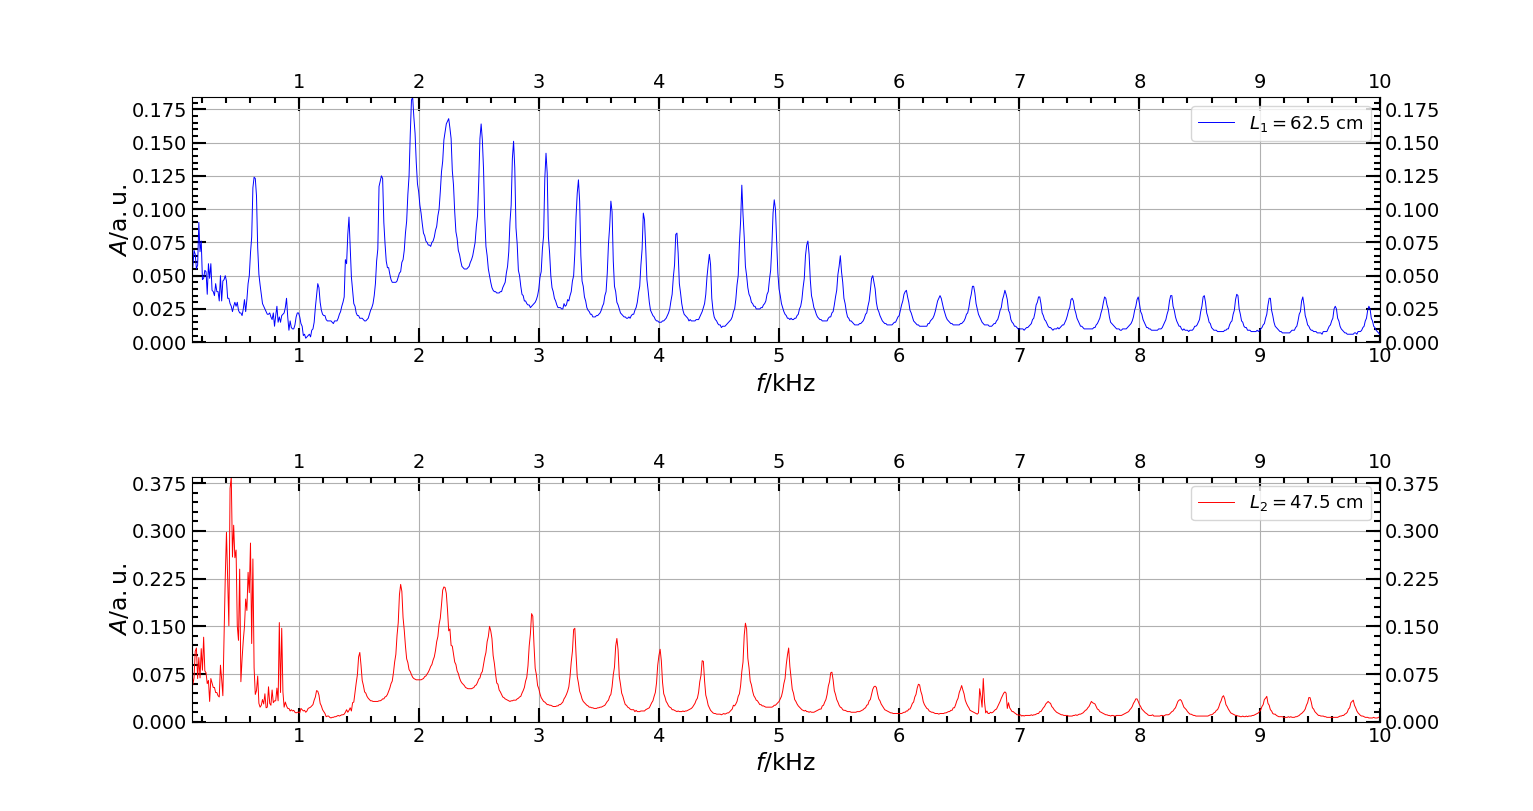
\includegraphics[width=0.9\textwidth]{421_Resonanzen.png} 
\caption{Frequenzspektrum für $L_1$ und $L_2$}
\end{figure} 
\[\]
\newpage
Es fällt auf, dass für die größere Länge die Abstände zwischen den Peaks kleiner sind. Dies hängt mit Gleichung (\ref{1}) zusammen. Umgestellt nach den Frequenzabständen $\Delta f$ der Peaks lautet diese nämlich:
\begin{align}
\Delta f = \frac{c}{2\,L} 
\end{align}
Unter der Annahme, dass die gleiche Schallgeschwindigkeit vorlag ist also $\Delta f$ umso größer, desto kleiner die Länge $L$. Außerdem sind diese immer äquidistant, was auch in obigem Plot zu erkennen ist.


Durch Durchnummerierung der ersten 20 Peaks mit $n=1,...,20$ konnten folgende Plots erstellt werden: 
\begin{figure}[h!]
\centering
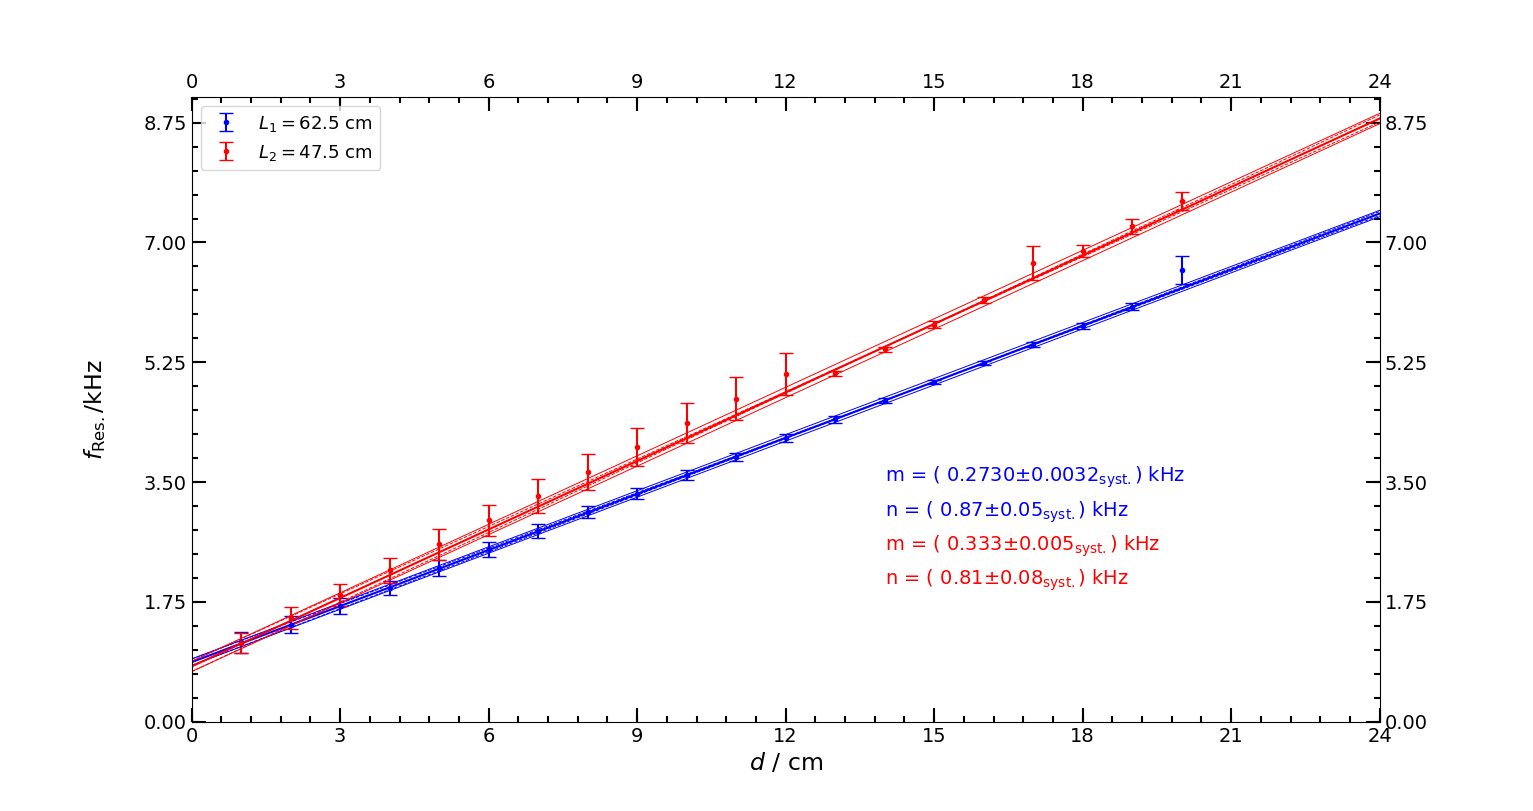
\includegraphics[width=0.85\textwidth]{421_systematische_Unsicherheiten.png}
\caption{Ausgleichsgerade mit systematischen Unsicherheiten}
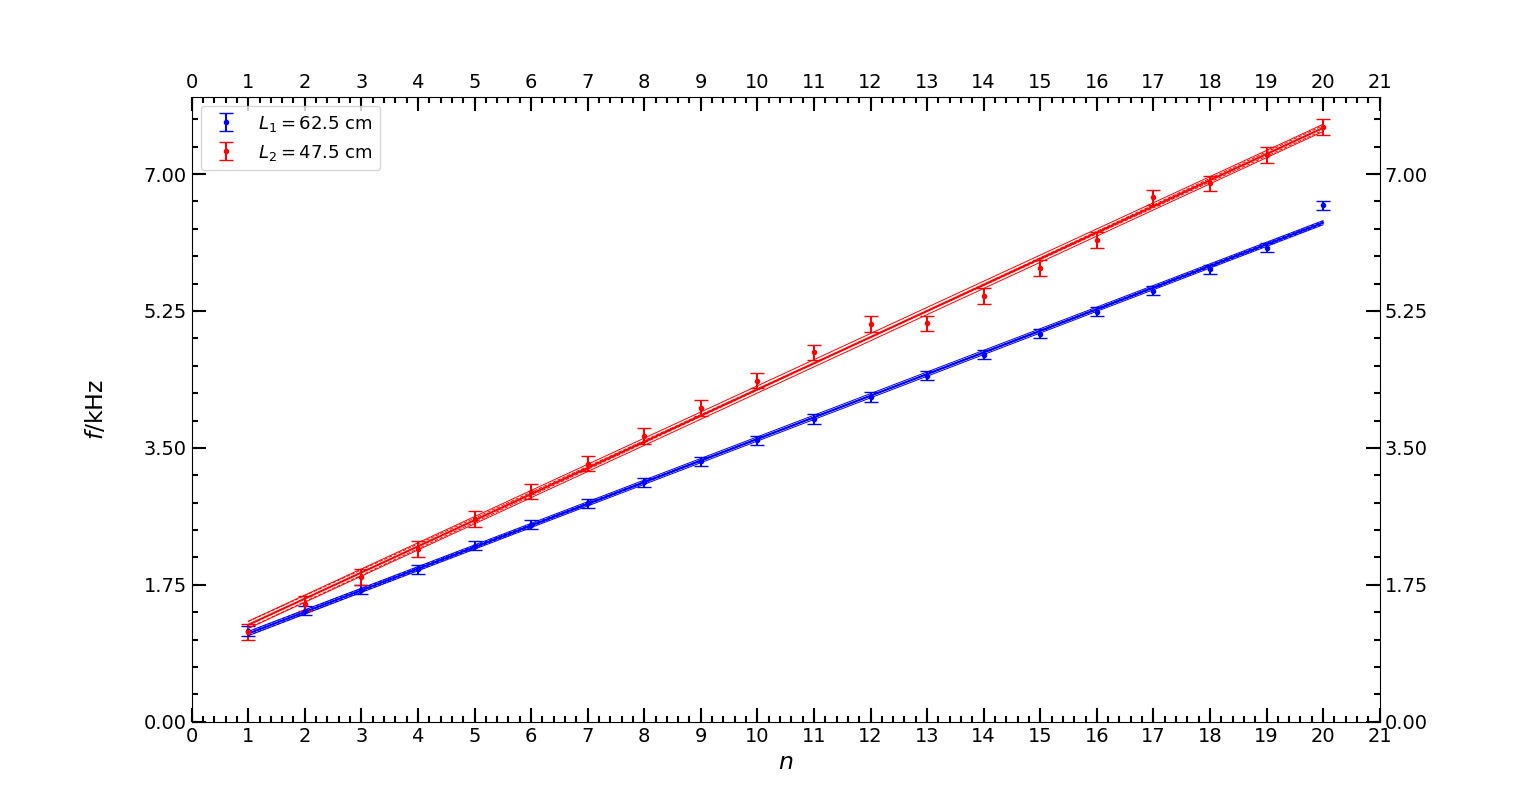
\includegraphics[width=0.85\textwidth]{421_statistische_Unsicherheiten.png}
\caption{Ausgleichsgerade mit statistischen Unsicherheiten}
\end{figure} 
\newpage
Er stellt die Resonanzfrequenz in Abhängigkeit von der Nummer $n$ mit systematischer bzw. statistischer Unsicherheit dar. Daraus kann die Schallgeschwindigkeit aufgrund des Zusammenhangs (\ref{schall}) aus dem Anstieg bestimmt werden:
\begin{align}
\label{schall} f = n \cdot\frac{c_{\mathrm{Schall}}}{2L}
\end{align}
Man erhält also die experimentellen Werte für die Schallgeschwindigkeit aus dem Anstieg, indem man diesen mit $2L$ multipliziert. In diesem Fall ergaben sich die Schallgeschwindigkeiten zu:
\begin{align}
c_{\mathrm{Schall}}^{\mathrm{experimentell}} =
  \begin{cases}
    343,4 \pm 2,8_{\mathrm{stat.}} \pm 4,0_{\mathrm{sys.}}  & \text{für} \ L_{1}  \\
	317,1 \pm 3,7_{\mathrm{stat.}} \pm 5,0_{\mathrm{sys.}} & \text{für} \ L_{2}
  \end{cases}
\end{align}
Schließlich kann man die experimentell ermittelten Werte mit dem aus der Theorie errechneten Wert vergleichen. Der Wert für $L_1$ stimmt sehr gut mit dem Wert aus der Theorie überein. Der Wert für $L_2$ liegt allerdings weit von dem theoretischen Wert entfernt, selbst wenn man von den maximalen Unsicherheiten ausgeht. Dies könnte daran liegen, dass wie bereits diskutiert, für die kürzere Länge die Peaks breiter sind. Dies erschwert es die genaue Lage des Maximums zu bestimmen und bewirkt also eine zusätzliche Abweichung von der tatsächlichen Peak-Frequenz.
\newline
\newline Analog zum Teilchen im unendlich hohen Potential Topf kommt es also zur Ausbildung stehender Wellen im Resonator. Allerdings sind die Peaks im Resonator bezüglich der Frequenz äquidistant und die Energien $E(n)$ sind proportional zu $n^2$, also nicht äquidistant.

\subsubsection{Theoretisches Modell und Reproduzierbarkeit}
Um die Reproduzierbarkeit der Messung zu untersuchen wurden mit Hilfe eines Fit-Programms für 8 Peaks in einem Frequenzbereich von $1,6$ kHz bis $4,5$ kHz ein Fit vorgenommen. Dies ist im folgenden Plot dargestellt: 
\begin{figure}[h!]
\centering
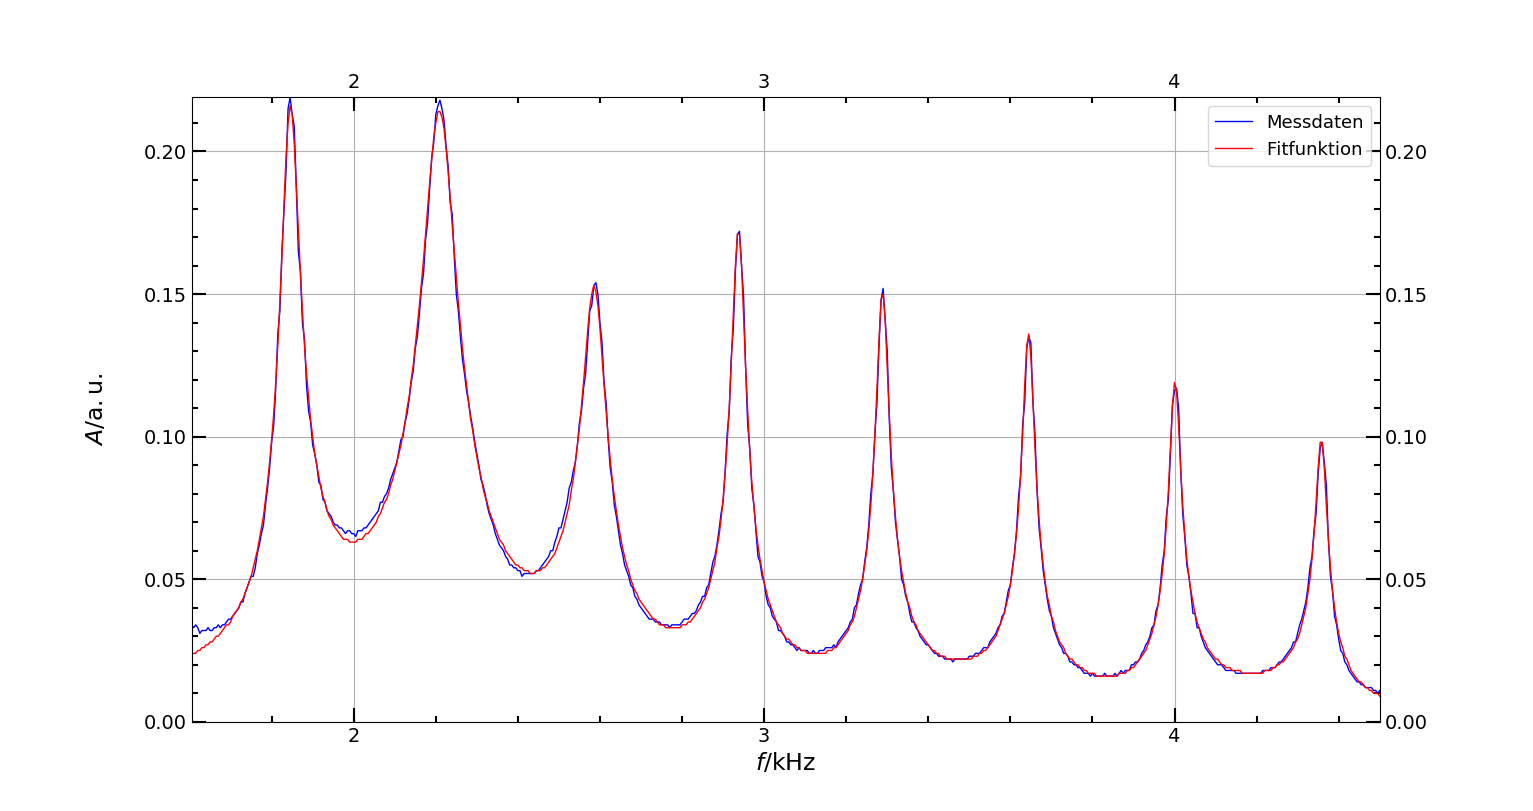
\includegraphics[width=0.7\textwidth]{Messung_L2_und_Fitfunktion.png}
\caption{Fit des theoretisches Modells zum experimentellen Spektrum}
\end{figure}
\newpage
Es ist also zu erkennen, dass dass das aufgenommene Frequenzspektrum sehr gut durch die im Fit-Programm verwendeten Gauß-Funktionen dargestellt werden können.
Somit ist die Reproduzierbarkeit und eine Übereinstimmung mit dem theoretischen Modell gegeben.

\subsection{Kugelresonator}
\subsubsection{Bestimmung der Resonanzfrequenzen und Winkelabhängigkeit der Wellenfunktion}
Nach Anpassung der Attentuator-Einstellung zur Signalabschwächung wurde ein Übersichtsspektrum zwischen $100$ Hz und $8$ kHz für einen Winkel $\alpha$ von $180^{\circ}$ (dies entspricht $\theta = 180^{\circ}$) aufgenommen. Dieses ist hier abgebildet: 
\begin{figure}[h!]
\centering
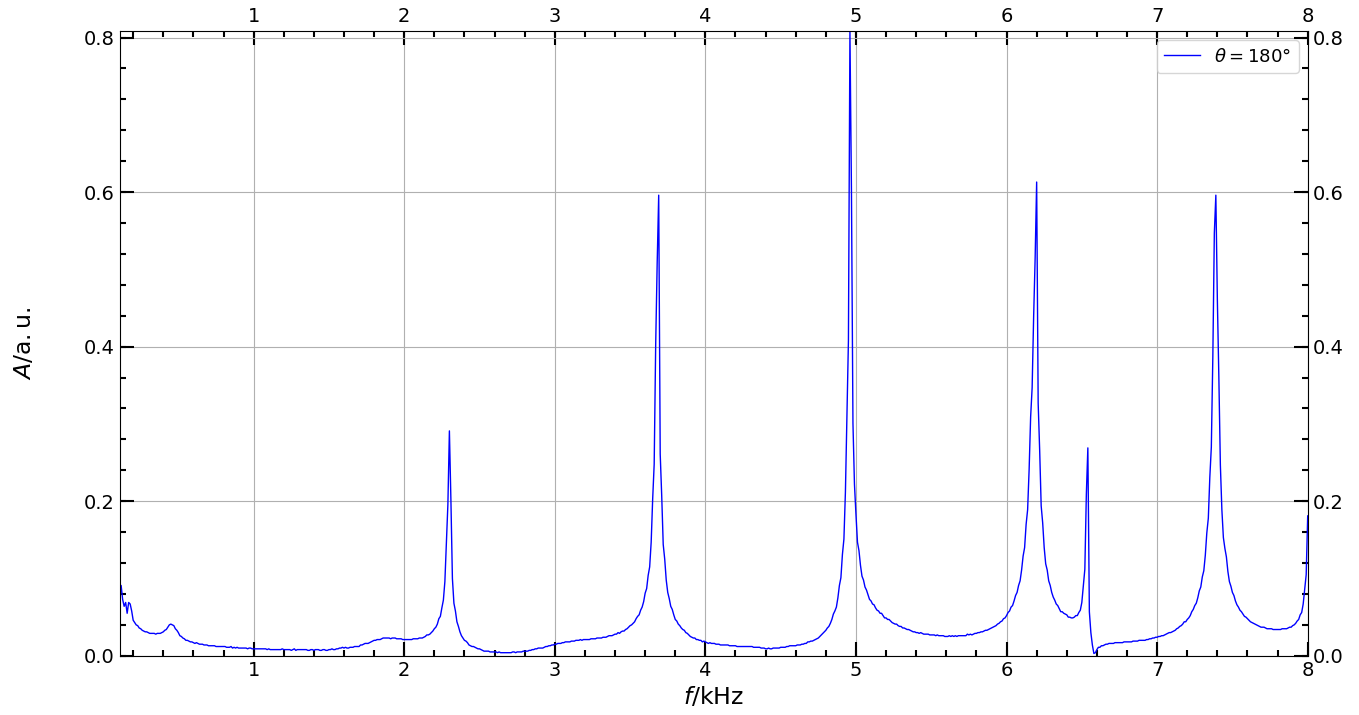
\includegraphics[width = 0.7\textwidth]{4311}
\caption{Übersichtsspektrum für $\alpha = \theta = 180^{\circ}$}
\end{figure} 
\newpage
Wieder ergaben sich Resonanzfrequenzen als Peaks. Diese lagen bei: $2300$ Hz, $3680$ Hz, $4970$ Hz, $6170$ Hz und $7420$ Hz.
Diese Messung wurde für weitere Winkel $\alpha$ von  $0^{\circ}$, $60^{\circ}$, $85^{\circ}$ und $120^{\circ}$ wiederholt. Nach der gegebenen Vorschrift in $\theta$ umgerechnet lauten diese: $90^{\circ}$; $104,48^{\circ}$; $117,16^{\circ}$ und $138,59^{\circ}$. Die 4 Spektren sind in folgendem Plot zur besseren Vergleichbarkeit zusammen dargestellt: \\\\
\begin{figure}[h!]
\centering
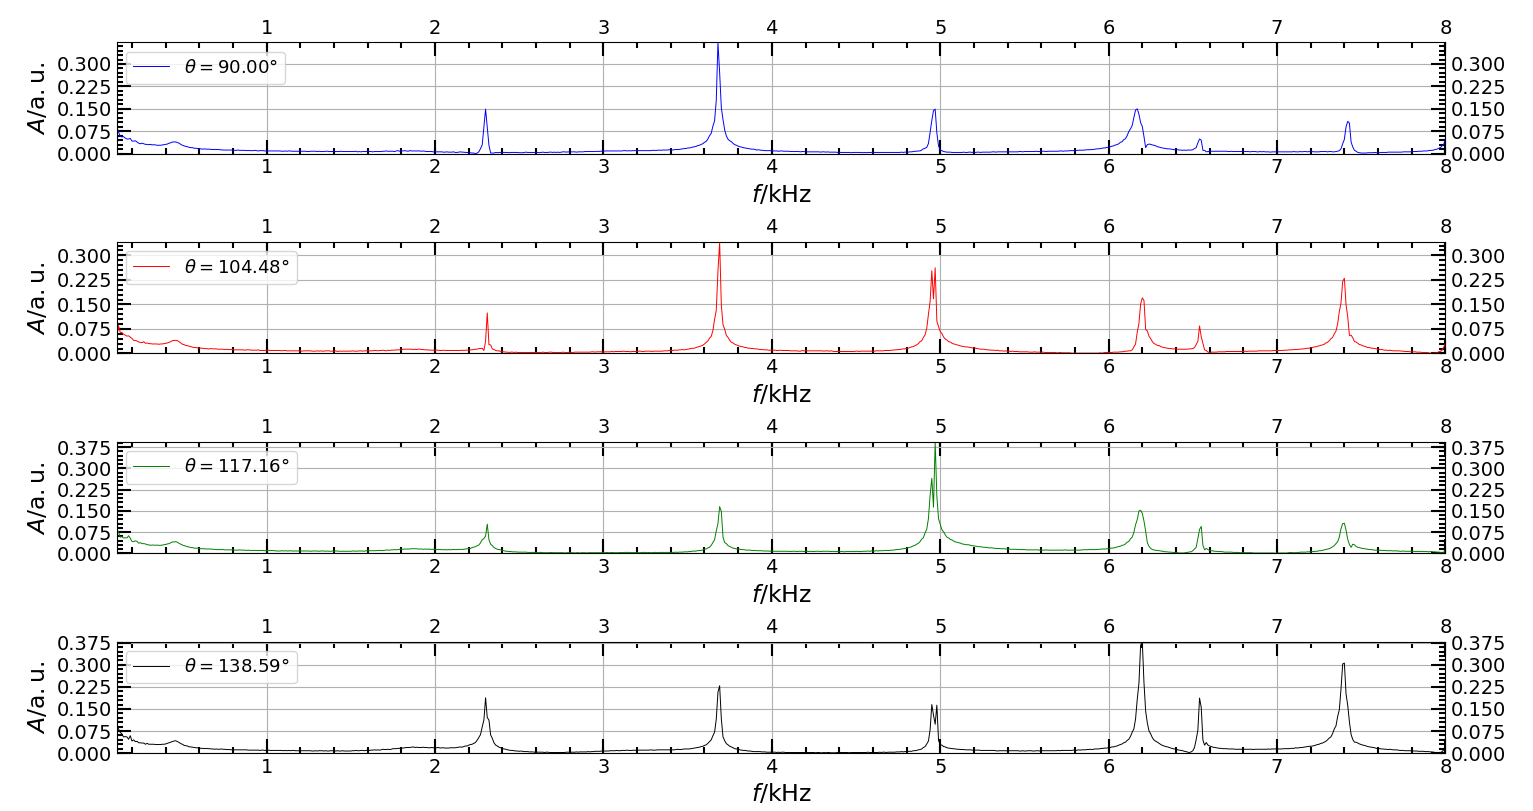
\includegraphics[width=\textwidth]{4312.png}
\caption{Frequenzspektren für verschiedene Winkel $\theta$}
\end{figure} \\\\
Die Peaks aller 4 Winkel sind mit ihren Amplituden in folgender Tabelle dargestellt: \\\\
\begin{table}[h!]\centering
\begin{tabular}{|c|c|c|c|c|} \hline
Nr. des Peaks & $\theta=90^{\circ}$ & $\theta=104,48^{\circ}$ & $\theta=117,16^{\circ}$ & $\theta=138,59^{\circ}$ \\ \hline
1 	& 0,149 & 0,124 & 0,103 & 0,188 	\\ \hline
2 	&  0,372 & 0,340 & 0,165 & 0,229	\\ \hline
2  	& 0,149 & 0,262 & 0,393 & 0,165 	 \\ \hline
4	& 0,150 	& 0,170 & 0,152 & 0,378  	 \\ \hline
5	& 0,108 &   0,230 & 0,106 & 0,306	 \\ \hline
\end{tabular}
\end{table} \\\\
Im Folgenden betrachten wir exemplarisch den zweiten Peak. Dieser entspricht $l=2$. Zudem haben wir ohne Symmetriebrechung immer den Fall $m=0$ vorliegen. An den Werten der Intensitäten ist zu erkennen, dass diese für $\theta = 90^{\circ}$ circa halb so groß ist wie für $\theta=180^{\circ}$. Außerdem sehen wir an den Diagrammen, dass zwischen $\theta=117,16^{\circ}$ und $\theta=138,59^{\circ}$ ein Minimum der Intensität erreicht werden muss. Dies hängt mit den Legendre-Polynomen zusammen. Für den zweiten Peak gilt es $P^{0}_{2}(\cos \theta)=\frac{1}{2}\,(3\,\cos^2\theta-1)$ zu betrachten. Dieses ist grafisch als grüner Graph in der folgenden Abbildung mit den ersten 5 Legendre-Polynomen dargestellt: \\\\
\begin{figure}[h!]
\centering
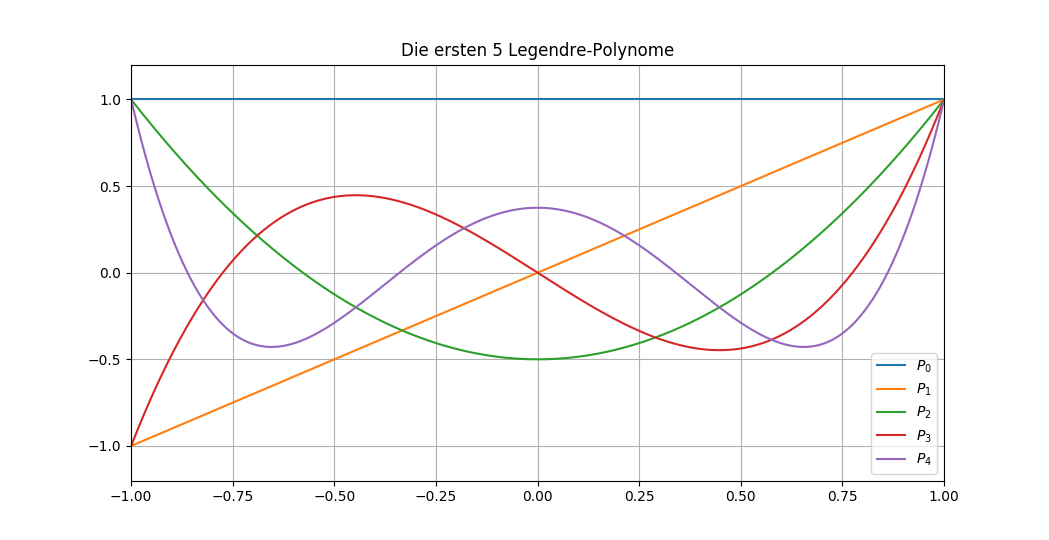
\includegraphics[width=\textwidth]{Legendre_Polynome.png}
\caption{Die ersten 5 Legendre-Polynome}
\end{figure} \\\\
Es ist also am Verlauf des Polynoms zu sehen, dass es bei $\cos(\theta)=1$ (entspricht $\theta = 180^{\circ}$) sein Maximum bei $1$ hat. Für $\cos(\theta)=0$ (entspricht $\theta = 90^{\circ}$) hat es ein Minimum mit Funktionswert $-0,5$. Dies korrespondiert mit der Beobachtung, dass die Intensität für $\theta = 90^{\circ}$ nur halb so hoch ist wie für $\theta = 180^{\circ}$. Das Legendre-Polynom hat für $\theta = 125,26^{\circ}$ einen Knoten. Dies ist in Einklang damit, dass die Intensität zwischen $\theta=117,16^{\circ}$ und $\theta=138,59^{\circ}$ ein Minimum hat.
\newline Letztendlich kann man folgern, dass die experimentellen Beobachtungen unter Berücksichtigung der hohen Sensibilität des Versuchsaufbaus gut mit der Theorie übereinstimmen.
\newpage
\subsubsection{Polardiagramme}
Durch die Messung des hochaufgelösten Spektrums ergibt sich folgendes Bild: 
\begin{figure}[h!]
\centering
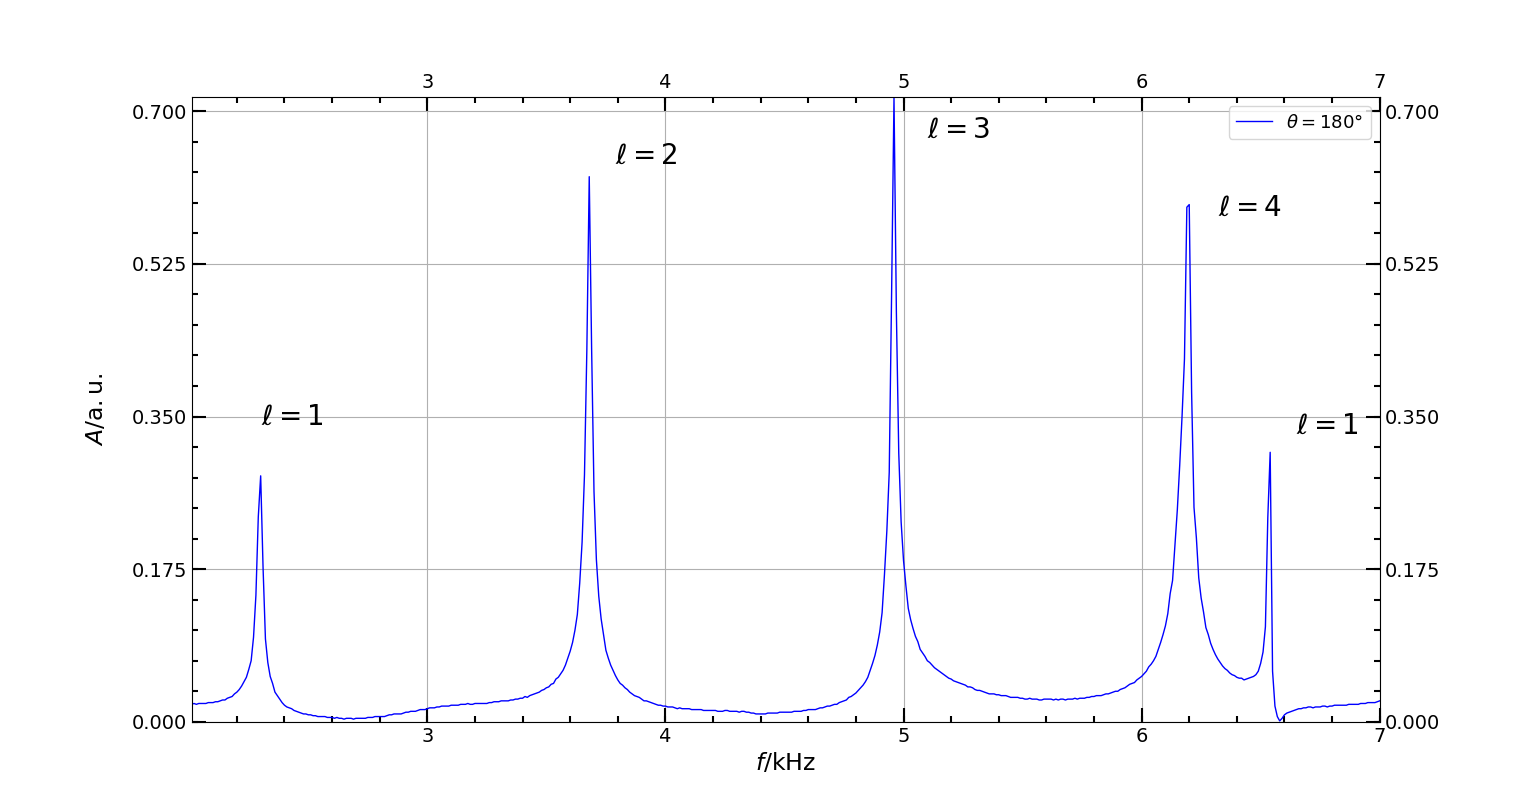
\includegraphics[width=\textwidth]{4321.png}
\caption{Hochaufgelöstes Spektrum für $\theta = 180^{\circ}$}
\end{figure} \\\\
Nun kann jeder Resonanzpeak einzeln angewählt werden und so für die jeweilige Resonanzfrequenz das Polardiagramm aufgenommen werden. Die so entstandenen Diagramme sind hier für die jeweiligen Peaks dargestellt:\\\\
\begin{minipage}{0.48 \textwidth} \centering
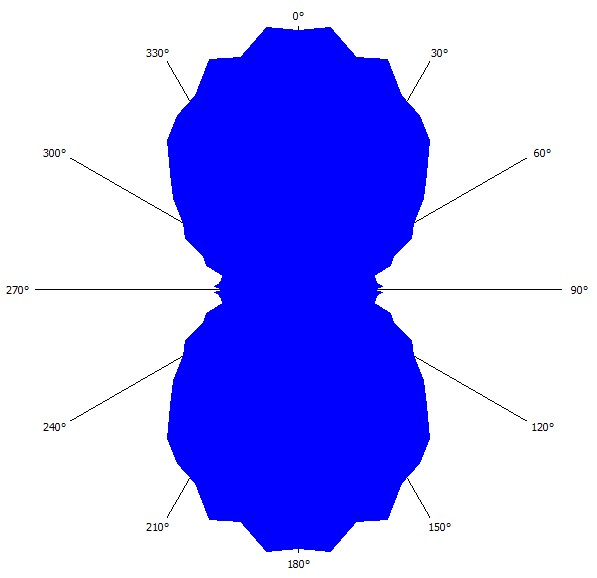
\includegraphics[scale=0.3]{432_Peak_1.jpg}
\captionof{figure}{Polardiagramm zu Peak 1}
\end{minipage}
\begin{minipage}{0.48 \textwidth} \centering
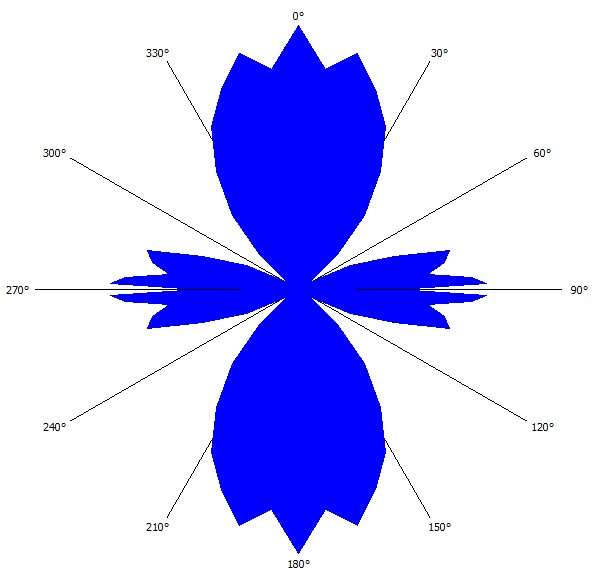
\includegraphics[scale=0.3]{432_Peak_2.jpg}
\captionof{figure}{Polardiagramm zu Peak 2}
\end{minipage}
\\\\
\begin{minipage}{0.48 \textwidth} \centering
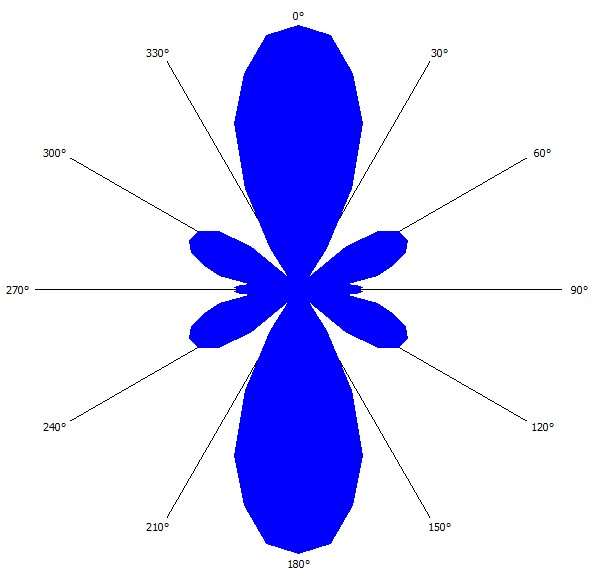
\includegraphics[scale=0.3]{432_Peak_3.jpg}
\captionof{figure}{Polardiagramm zu Peak 3}
\end{minipage}
\begin{minipage}{0.48 \textwidth} \centering
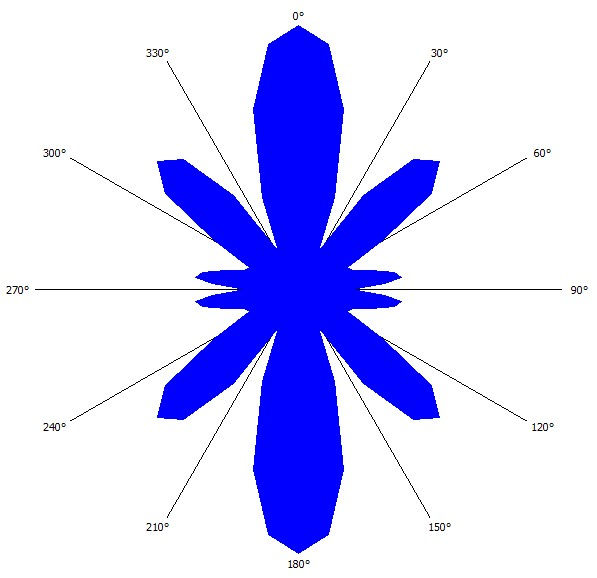
\includegraphics[scale=0.3]{432_Peak_4.jpg}
\captionof{figure}{Polardiagramm zu Peak 4}
\end{minipage}
\\\\
\begin{minipage}{0.48 \textwidth} \centering
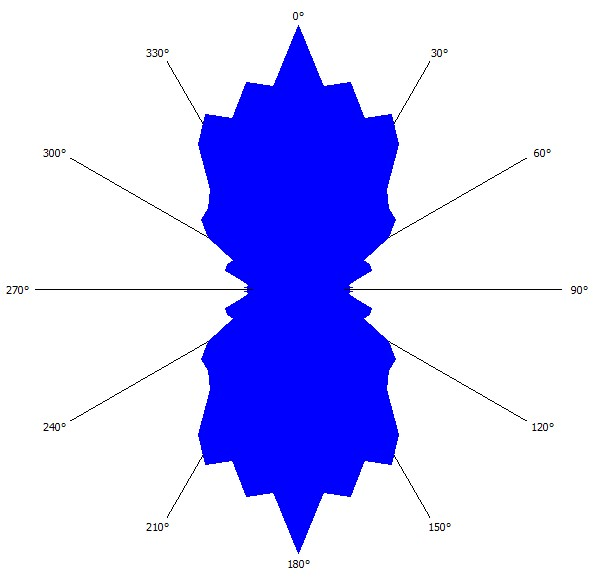
\includegraphics[scale=0.3]{432_Peak_5.jpg}
\captionof{figure}{Polardiagramm zu Peak 5}
\end{minipage}
\\\\
Ein Vergleich mit den Kugelflächenfunktionen des Programms PlotYlm.exe liefert dann die bereits im Diagramm angegebene Zuordnung der l-Quantenzahlen.
\newline Als Fazit kann man also sagen, dass die gemessenen Polardiagramme den theoretischen Fakt untermauern, dass die winkelabhängigen Gleichungen für das Wasserstoffatom und den Kugelresonator die gleiche Lösung haben, die Kugelflächenfunktionen. Außerdem steigt mit der Frequenz auch die l-Quantenzahl. Beim Wasserstoffatom muss zuerst die Hauptquantenzahl $n$ erhöht werden, um bestimmte l-Zustände erreichen zu können, da $l$ von $0$ bis $n-1$ läuft. Analog dazu steigt mit der Frequenz die l-Quantenzahl in diesem Versuch. Jedoch ist dies eher eine qualitative als eine quantitative Gemeinsamkeit.

\subsection{Symmetriebrechung}
Für diesen Teilversuch wurde zuerst das Spektrum der ersten drei Peaks für den Kugelresonator gemessen. Der dazu ausgewählte Frequenzbereich war $2,0$ kHz bis $5,6$ kHz in Frequenzschritten von $5$ Hz bei $\alpha = 180^{\circ}$. Dieses Spektrum sieht wie folgt aus:
\\\\
\begin{figure}[h!]
\centering
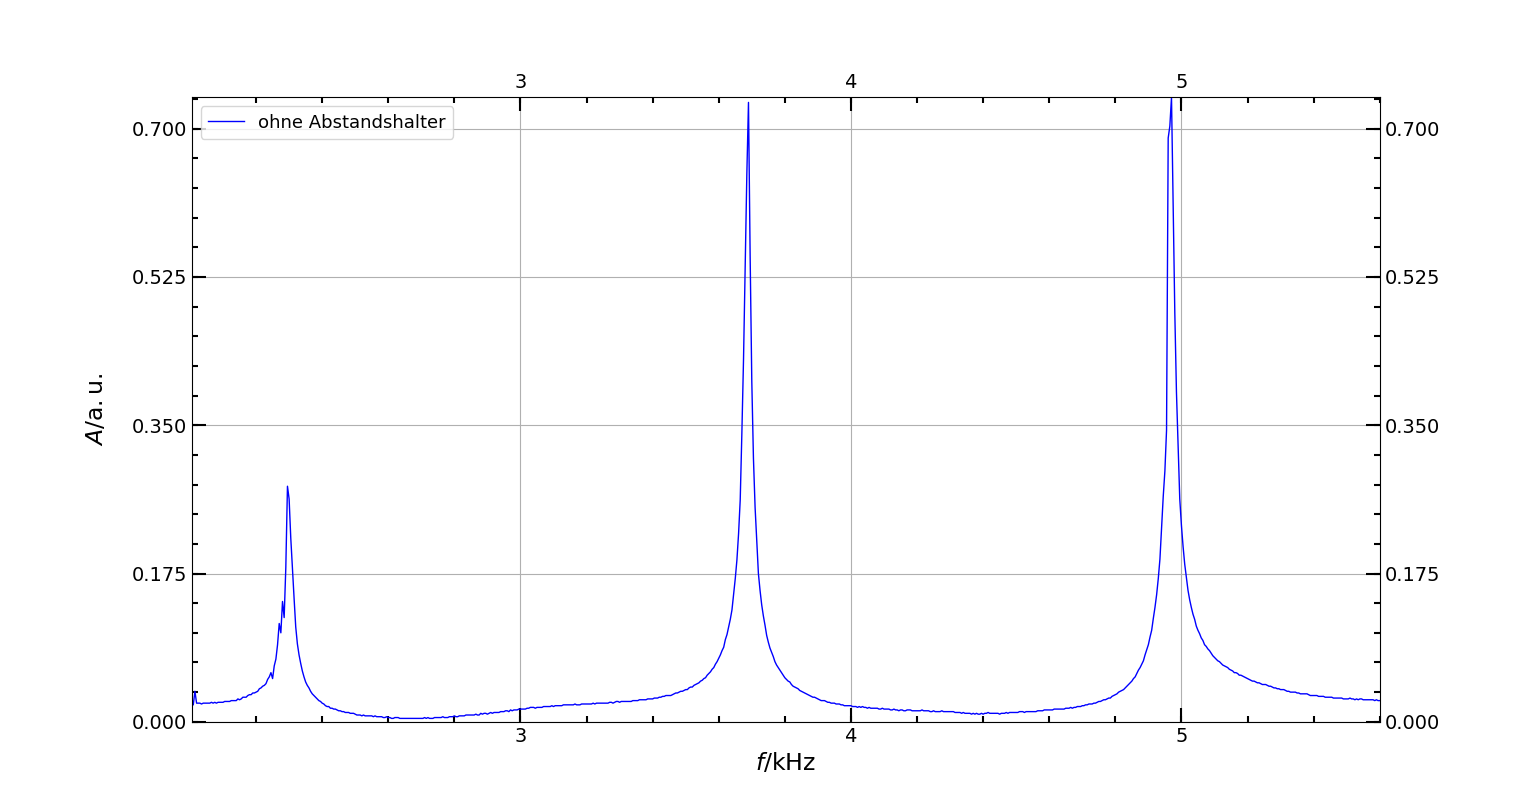
\includegraphics[width=\textwidth]{441_Uebersicht.png}
\caption{Spektrum der ersten drei Peaks des Kugelresonators }
\end{figure}
\\\\
Selbige Messung wurde unter Einfügen eines Abstandshalterringes mit jeweiliger Dicke d wiederholt. Dies ergab folgende Spektren:
\newpage
\begin{figure}[h!]
\centering
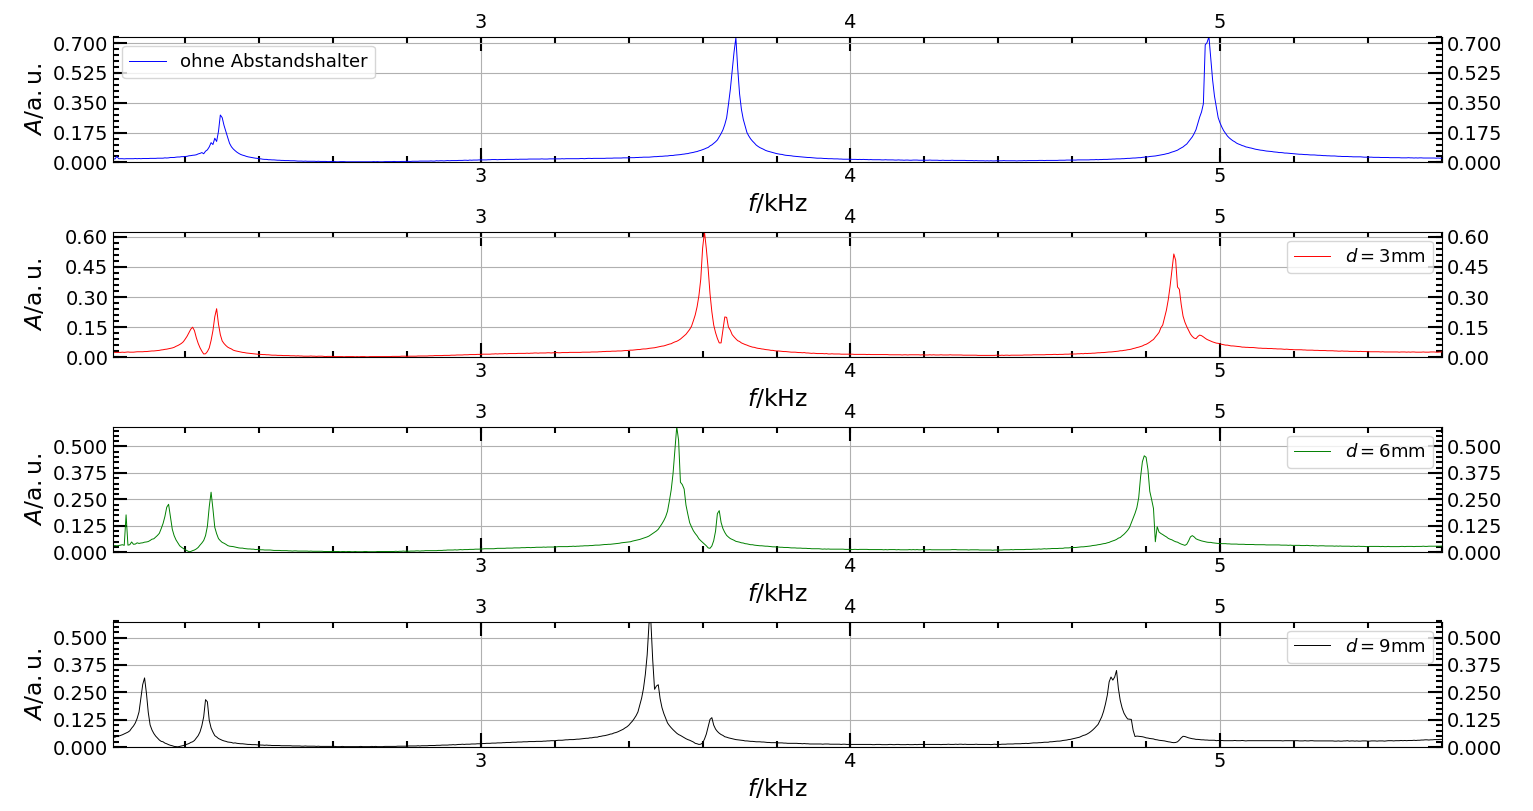
\includegraphics[width=\textwidth]{442_und_443.png}
\caption{Spektrum der ersten drei Peaks mit und ohne Abstandshalterring}
\end{figure}
Die Resonanzpeaks ohne Abstandshalter, die jeweils eine l-Quantenzahl repräsentieren, spalten sich also in zwei Peaks auf. Dies ist Folge der Symmetriebrechung durch Einfügen des Abstandshalterringes. Für eine zunehmende Dicke d wir die Symmetrie stärker gebrochen und die Aufspaltung nimmt mehr und mehr zu. Diese Aufspaltung repräsentiert die magnetische Quantenzahl $m$. Jedem durch Aufspaltung entstandenen Peak kann die gleiche Quantenzahl $l$ und eine unterschiedliche Quantenzahl $m$ zugeordnet werden. Jedoch ist zu beachten, dass trotzdem noch eine Entartung von $m$ und $-m$ aufgrund der verbleibenden Symmetrieeigenschaften bestehen bleibt. Somit wird eigentlich nur $|m|$, also eine positive Magnetquantenzahl, zugeordnet.
\\
Um diese Aufspaltung nun exemplarisch genauer zu untersuchen wurden die Peaks mit $l=1$ ausgewählt, um noch einmal ein hochaufgelöstes Spektrum aufzunehmen um unter Auswahl der aufgespaltenen Peakfrequenzen Polardiagramme aufzunehmen. Das Spektrum ist folgendes: 
\newpage
\begin{figure}[h!]
\centering
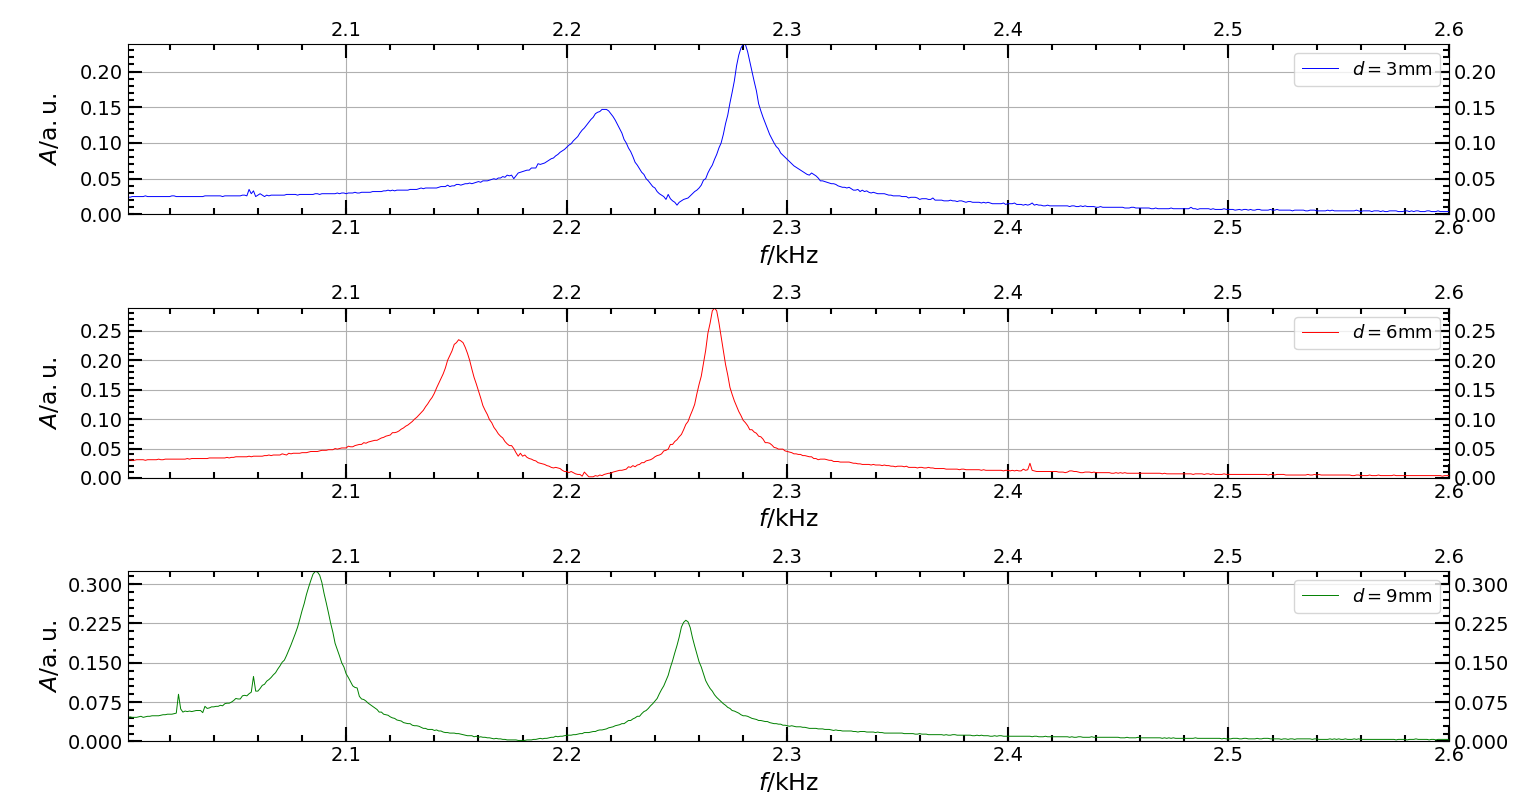
\includegraphics[width=\textwidth]{444.png}
\caption{Hochaufgelöstes Spektrum der Peaks mit $l=1$}
\end{figure}
Hier sieht man die zunehmende Aufspaltung bei zunehmendem $d$ noch einmal etwas deutlicher.
\newline Die bei den Peakfrequenzen aufgenommen Polardiagramme bei $d=9$mm sind dann diese:
\\\\
\begin{minipage}{0.48 \textwidth} \centering
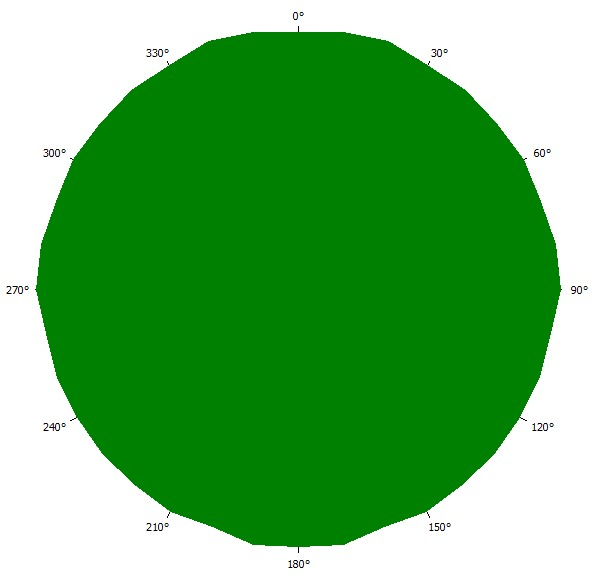
\includegraphics[scale=0.3]{445_l1_linker_Peak.jpg}
\captionof{figure}{Polardiagramm linker Peak für $l=1$}
\end{minipage}
\begin{minipage}{0.48 \textwidth} \centering
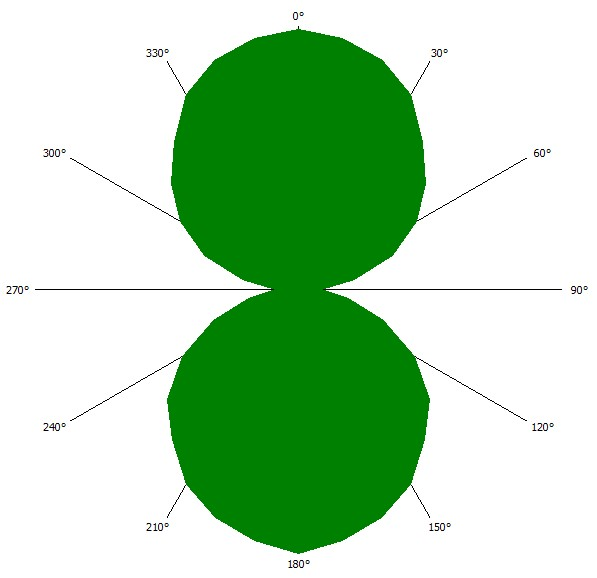
\includegraphics[scale=0.3]{445_l1_rechter_Peak.jpg}
\captionof{figure}{Polardiagramm rechter Peak für $l=1$}
\end{minipage}
\\\\
Ein Vergleich mit den Funktionen aus PlotYlm.exe liefert dann, dass dem Bild zum linken Peak ein $m$ von 0 und dem rechten Peak ein $|m|$ von 1 zugeordnet werden kann. 
\newline Selbiges Vorgehen wurde nun für $l=2$ wiederholt. Diese Polardiagramme sehen so aus:
\\\\
\begin{minipage}{0.48 \textwidth} \centering
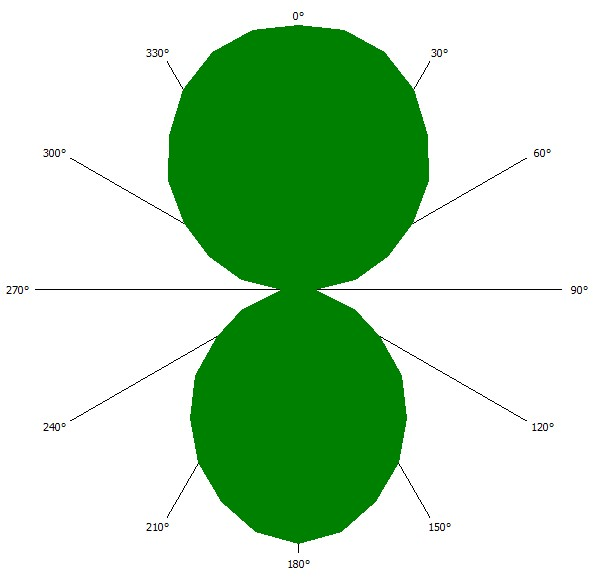
\includegraphics[scale=0.3]{445_l2_linker_Peak.jpg}
\captionof{figure}{Polardiagramm linker Peak für $l=2$}
\end{minipage}
\begin{minipage}{0.48 \textwidth} \centering
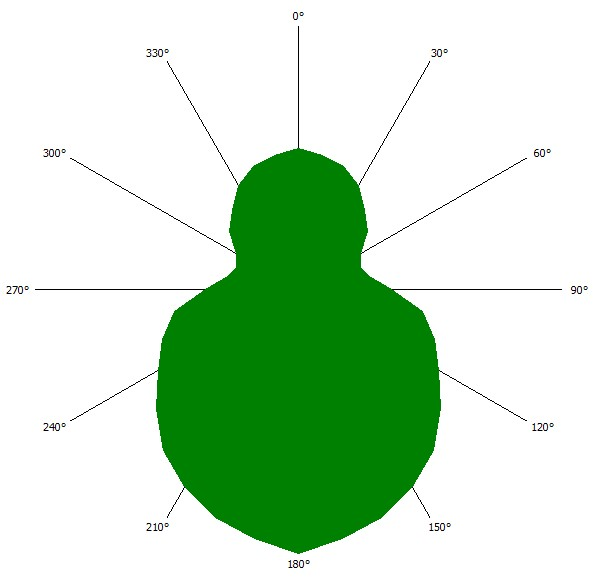
\includegraphics[scale=0.3]{445_l2_mittlerer_Peak.jpg}
\captionof{figure}{Polardiagramm mittlerer Peak für $l=2$}
\end{minipage}
\\\\
\begin{minipage}{0.48 \textwidth} \centering
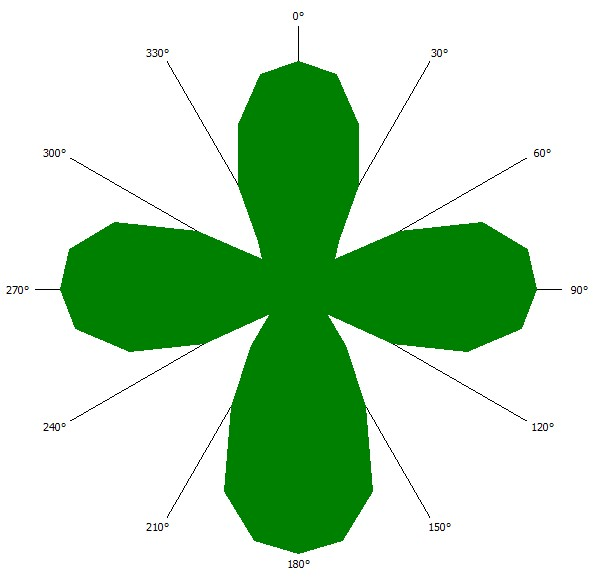
\includegraphics[scale=0.3]{445_l2_rechter_Peak.jpg}
\captionof{figure}{Polardiagramm rechter Peak für $l=2$}
\end{minipage}
\\\\
Hier ergibt die Zuordnung mit Hilfe des Programms für den mittleren Peak $m=0$, für den linken Peak $|m|=2$ und für den rechten Peak $|m|=1$.
\newline Die grafische Darstellung beider Peaks mit Hilfe des Tupels $(l,m)$ ergibt sich also zu:
\\\\
\begin{figure}[h!]
\centering
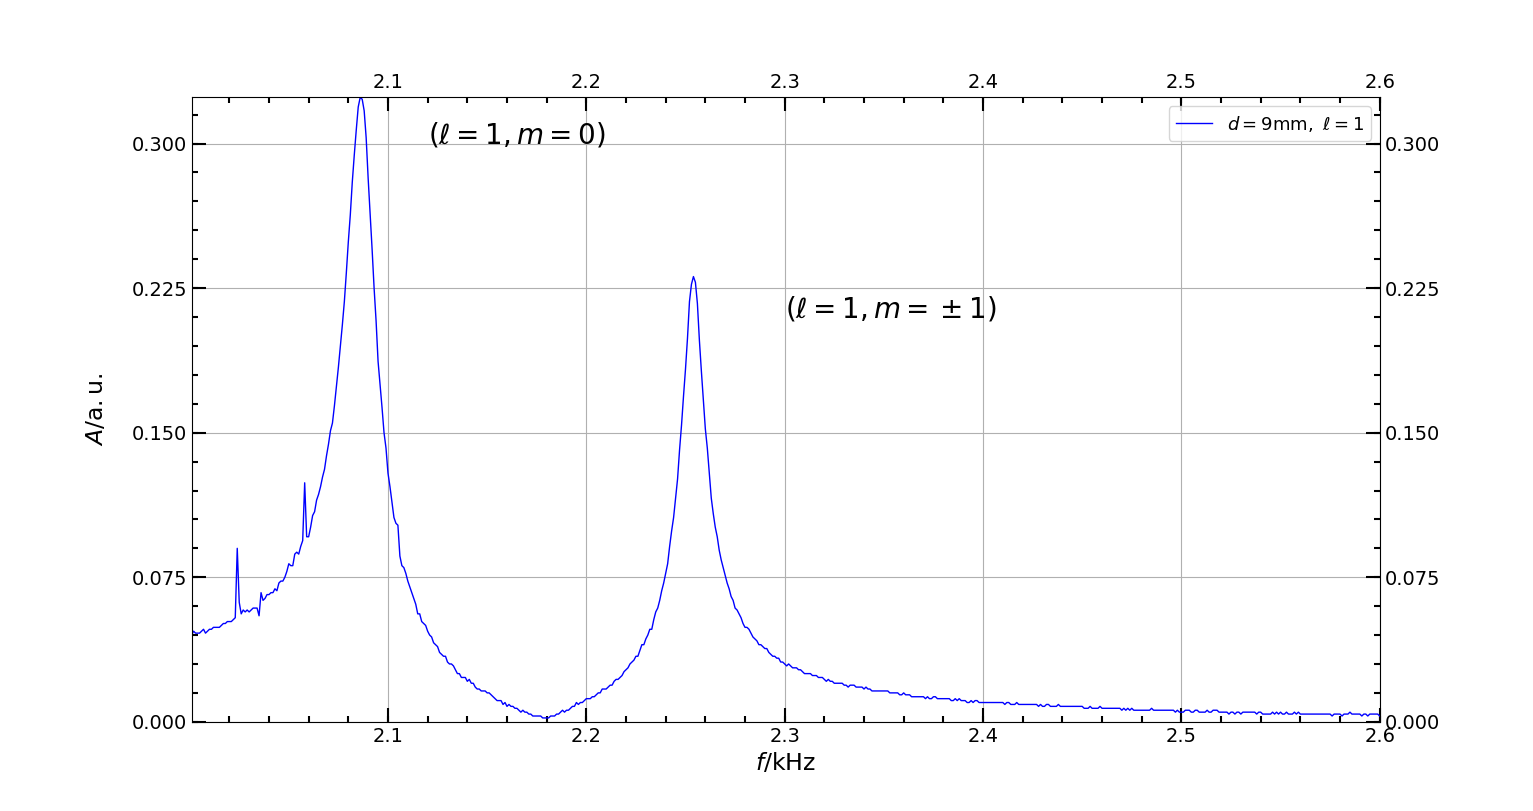
\includegraphics[width=\textwidth]{445_fuer_l_gleich_1.png}
\caption{Darstellung $(l,m)$ für $l=1$}
\end{figure}
\begin{figure}[h!]
\centering
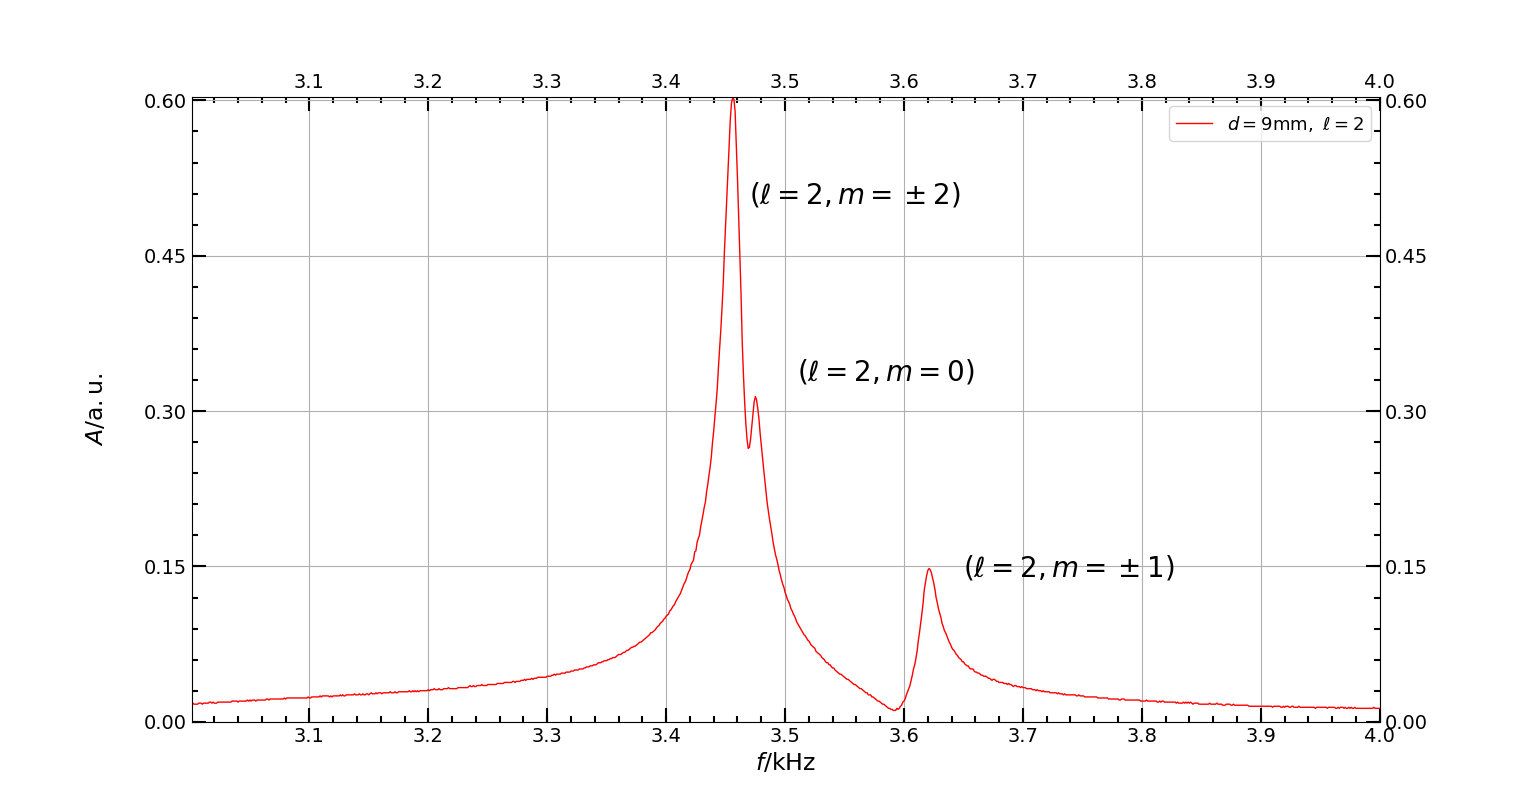
\includegraphics[width=\textwidth]{445_fuer_l_gleich_2.png}
\caption{Darstellung $(l,m)$ für $l=2$}
\end{figure}
\\\\


\subsection{Analogie zum Wasserstoffmolekül}
Um die Analogie zum Wasserstoffmolekül herzustellen, wurden 2 sphärische Resonatoren gekoppelt. Vergleichend ist hier das Spektrum für einen sphärischen Resonator (Atom) und zwei gekoppelte sphärische Resonatoren (Molekül) dargestellt:
\\\\
\begin{figure}[h!]
\centering
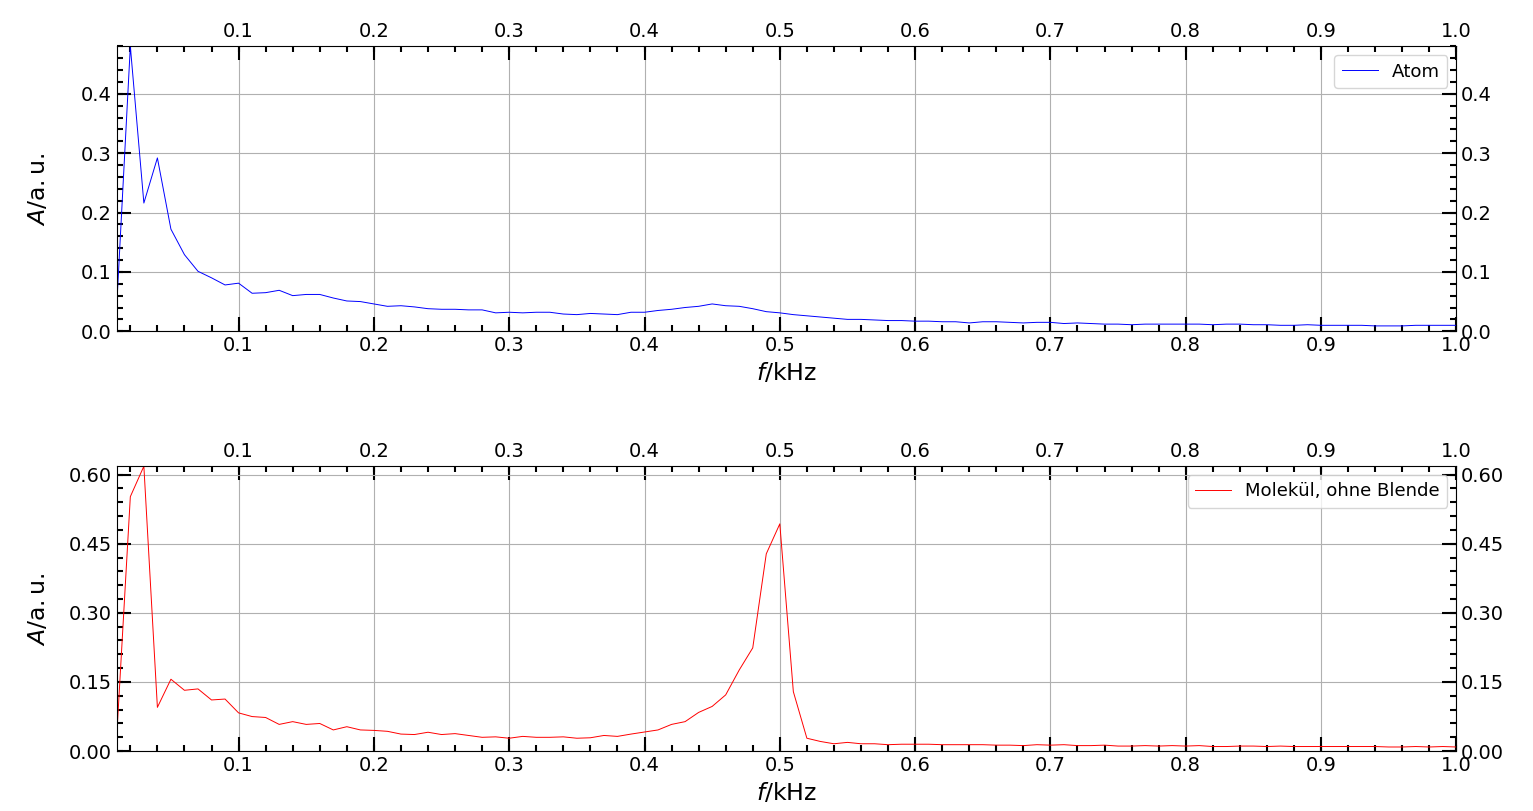
\includegraphics[width=\textwidth]{451.png}
\caption{Spektrum für einen und 2 gekoppelte sphärische Resonatoren}
\end{figure}
\\\\
Man kann also erkennen, dass man für ein Molekül ohne Blende, das heißt ohne Beeinflussung der Kopplungsstärke, einen zusätzlichen Peak bei ca. $0,5$ kHz erhält. Dies kann wieder über die Resonanzbedingung begründet werden. Für zwei Kugeln erhalten wir dieselbe Bedingung wie für eine Kugel, nur mit der doppelten Länge $2\,L$:
\begin{align}
L=n\,\frac{\lambda}{4}
\end{align}
Dadurch erhalten wir dieselben Resonanzen wie für den einzelnen Kugelresonator und noch zusätzliche Resonanzen der Form $\frac{\lambda}{4}$, $\frac{3\, \lambda}{4}$ usw. 
\\\\
Durch Einfügen einer Irisblende des Durchmessers $d$ wird die Kopplungsstärke verändert. Die zugehörigen Spektren für verschiedene Werte von $d$ sind folgende:
\\\\
\begin{figure}[h!]
\centering
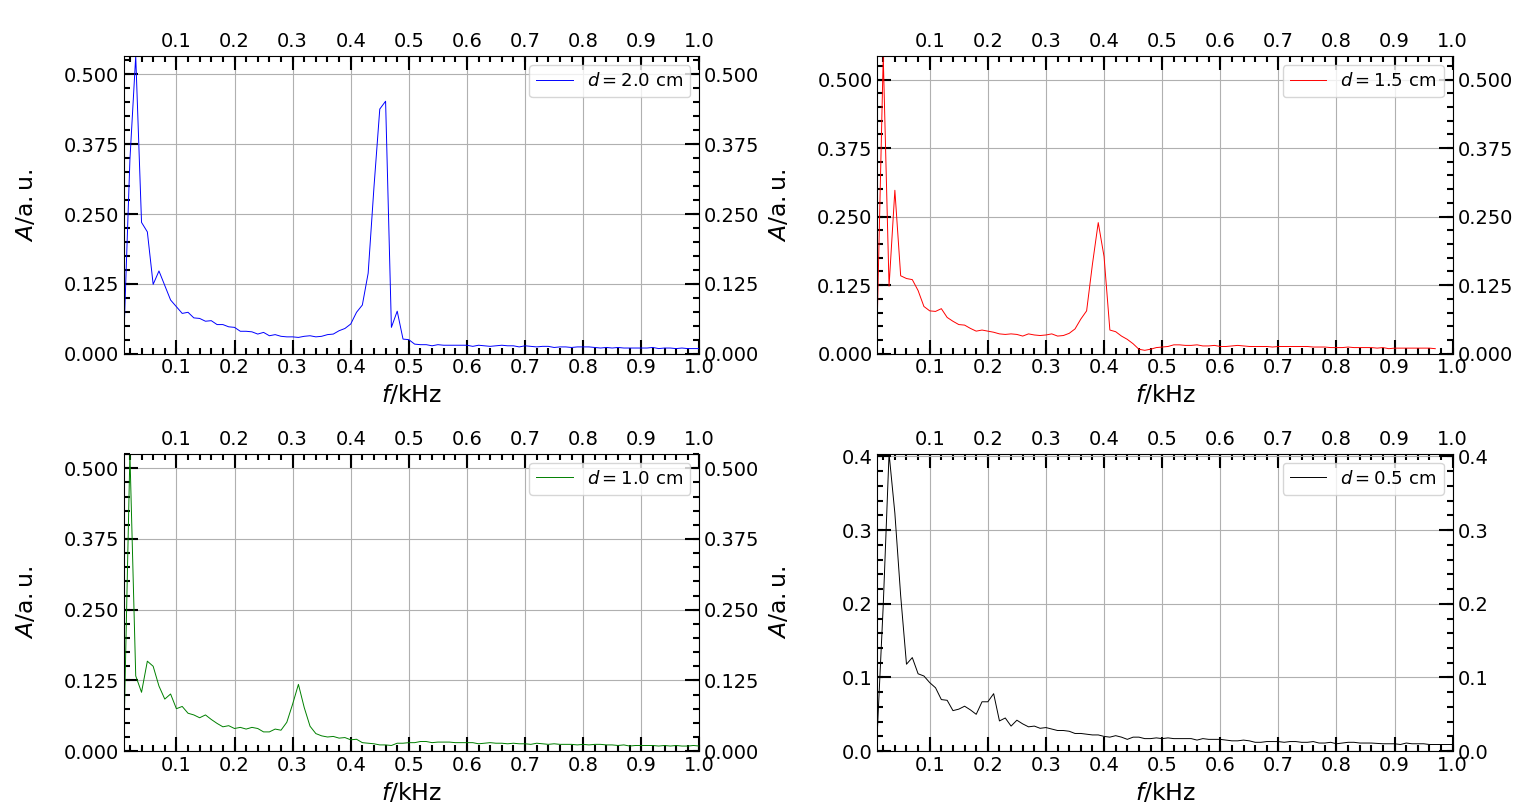
\includegraphics[width=\textwidth]{451_Molekuel_fuer_verschiedene_Blenden.png}
\caption{Spektrum des Moleküls für verschiedene Irisblenden}
\end{figure}
\newpage
Es lässt sich also erkennen, dass für einen kleiner werdenden Irisdurchmesser $d$ die zweiten Peaks immer kleiner werden. Zudem befinden sich die Peaks immer weiter links von den $0,5$ kHz. Diese Phänomene treten auf, da für kleinere Durchmesser $d$ die Kopplung immer schwächer wird und für schwache Kopplungen können die zwei Resonatoren separat betrachtet werden. Geht $d$ also gegen $0$, kommt als Grenzwert dafür das Spektrum für einen einzelnen sphärischen Resonator heraus. Macht man $d$ aber größer erhält man irgendwann das gleiche Bild wie für die zwei gekoppelten Resonatoren ohne Blende.
\newline Den Fakt des Nach-Links-Wanderns des Peaks für kleiner werdende Werte von $d$ kann man in Form eines Plots der Peakfrequenz in Abhängigkeit von $d$ darstellen:
\\\\
\begin{figure}[h!]
\centering
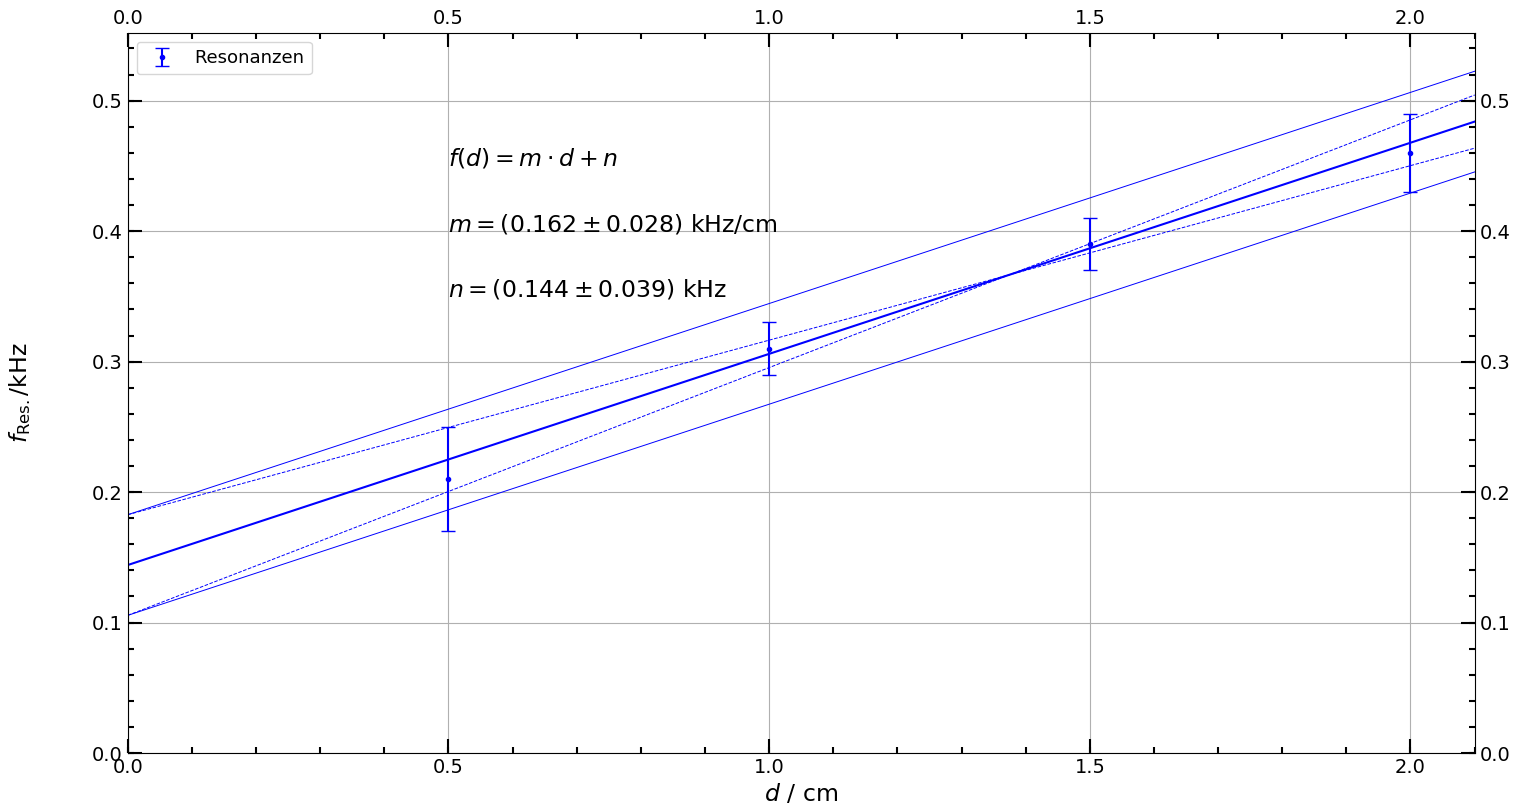
\includegraphics[width=0.6\textwidth]{451_Resonanzen_ueber_Irisdurchmesser.png}
\caption{Resonanzfrequenzen in Abhängigkeit vom Irisdurchmesser}
\end{figure}
\\\\
Es ist ein linearer Zusammenhang zu erkennen, bei dem die Ausgleichsgerade durchgelegt wurde. Die zur Geradengleichung gehörenden Parameter sind ebenfalls in dem Diagramm angegeben. Die Lage des zusätzlich entstandenen Resonanzpeaks als Charakteristikum der Kopplung hängt also linear von $d$, welches stellvertretend für die Kopplungsstärke steht, ab.
\newline 
\newline Der zweite Teil der Aufgabe ist die Aufnahme eines Polardiagramms für $d=20$mm. Dieses ist hier abgebildet:
\\\\
\begin{figure}[h!]
\centering
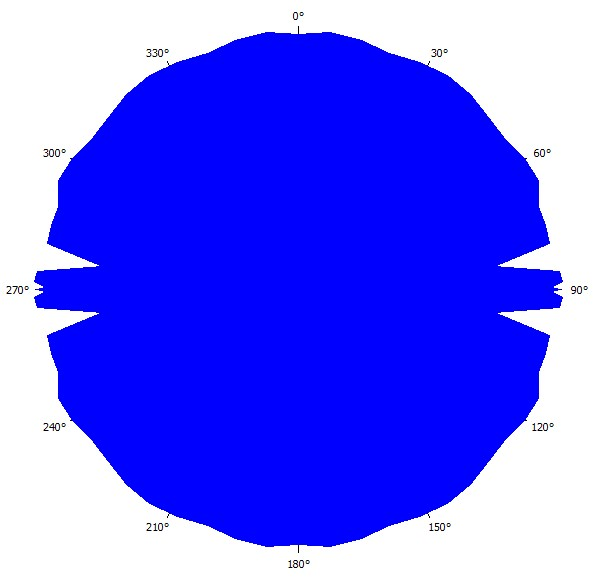
\includegraphics[width=0.4\textwidth]{452.jpg}
\caption{Polardiagramm des Moleküls für $d=20$mm}
\end{figure}
\\\\
Die entstandene Grafik zeigt also, dass das Molekül achsensymmetrisch ist. Deshalb entsteht eine Figur, die wie ein s-Orbital aussieht. Dies liegt daran, dass ein Molekül bestehend aus zwei identischen Atomen mit Hilfe von zwei identischen Kugelresonatoren simuliert wird.
\\\\
Im letzten Aufgabenteil galt es hochaufgelöste Spektren für die Resonanz bei $2300$ Hz für verschiedene Winkel $\varphi$ aufzunehmen. Diese Spektren sind hier abgebildet:
\newpage
\begin{figure}[h!]
\centering
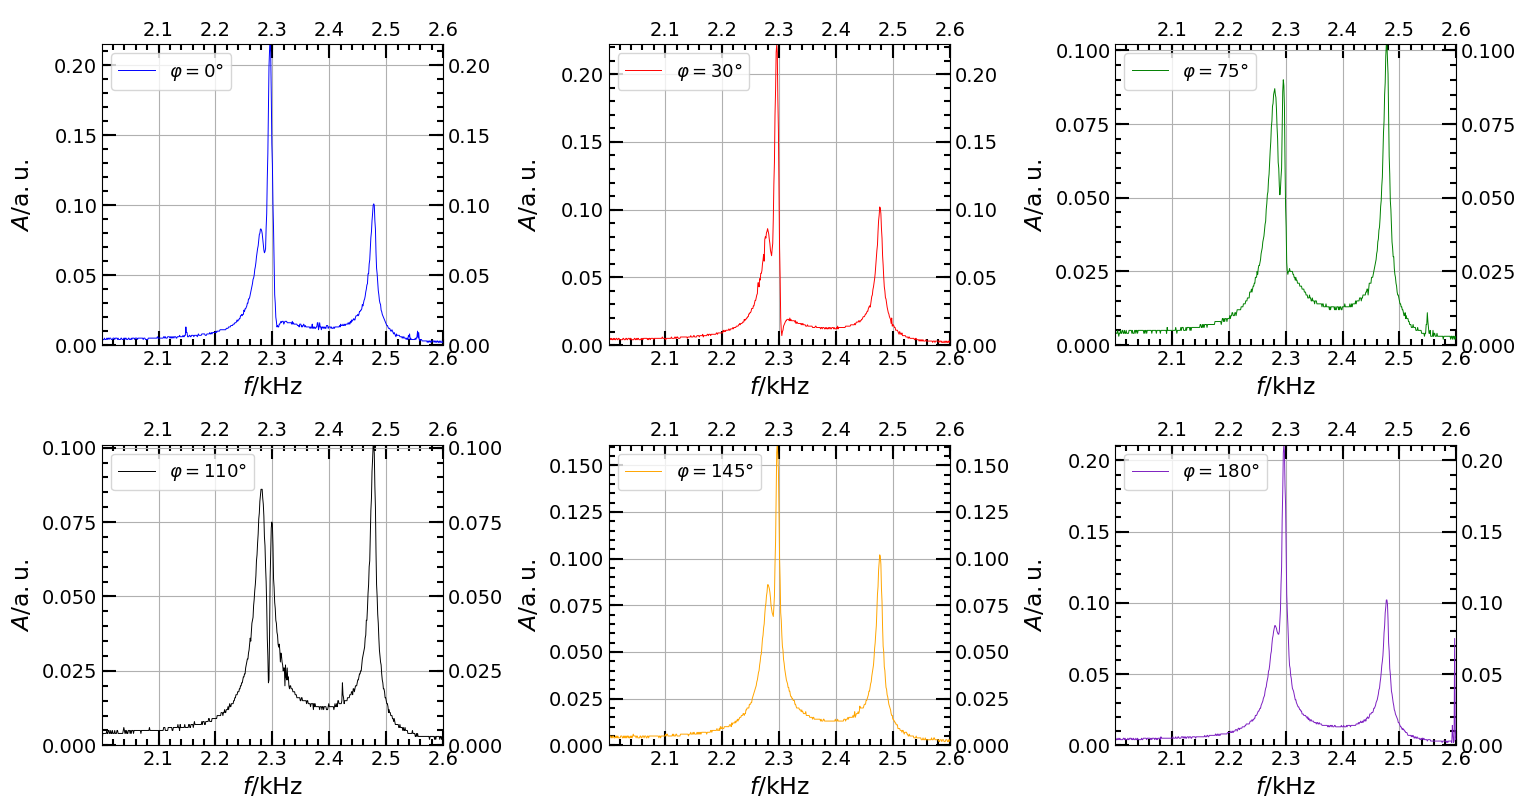
\includegraphics[width=\textwidth]{453.png}
\caption{Hochaufgelöste Spektren für verschiedene $\varphi$}
\end{figure}
Dies kann nun mit dem Spektrum für ein Atom verglichen werden. Da wir den Peak um $2300$ Hz untersuchen, handelt es sich im Vergleich mit dem Atom um einen molekularen Zustand, der vom atomaren $l=1$ - Zustand abgeleitet ist.
%grund für aufspaltung
In jedem der Diagramme sind 3 Peaks zu sehen. Diese können Molekülorbitalen zugeordnet werden.
Dem Peak, der sich jeweils ganz rechts befindet kann $\sigma_{\mathrm{antibindend}}$ zugeordnet werden und der Peak ganz links ist jeweils $\sigma_{\mathrm{bindend}}$. Für $\varphi=0^{\circ}$ liegt der mittlere Peak bei $2296$ Hz und für $\varphi=180^{\circ}$ liegt er bei $2297$ Hz. Diesen kann jeweils ein $\pi$-Orbital zugeordnet werden. Für $2296$ Hz ist es $\pi_{\mathrm{bindend}}$ und für $2297$ Hz ist es $\pi_{\mathrm{antibindend}}$. Die Zuordnung zu $\pi$ bzw. $\sigma$ und zu bindend bzw. antibindend erfolgte in Analogie zur Quantenmechanik. Die bindenden Orbitale liegen energetisch niedriger und sind deshalb in diesem Spektrum auch weiter links aufzufinden. Aber auch hier ist es, wie in der Quantenmechanik so, dass die $\pi$-Orbitale energetisch nah beieinander liegen und so schwer zu unterscheiden sind.

\subsection{Analogie zum 1D-Festkörper}
\subsubsection{Röhrenresonator mit Irisblenden}
Zuerst wurde ein Übersichtsspektrum für die Resonatorlängen $400$ mm und $600$ mm aufgenommen:
\\\\
\begin{figure}[h!]
\centering
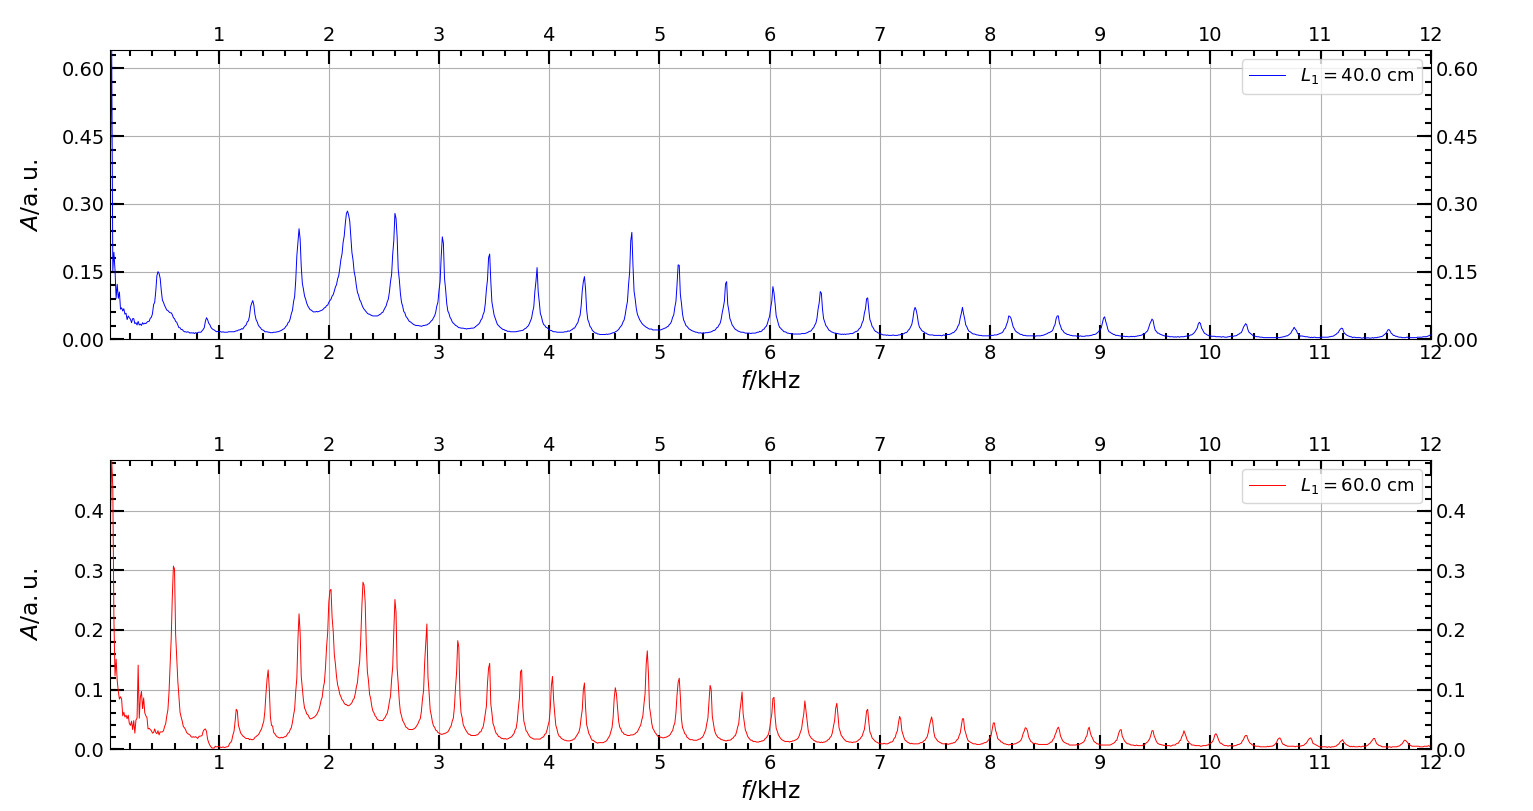
\includegraphics[width=\textwidth]{4611.png}
\caption{Übersichtsspektrum für die Resonatorlängen $400$ mm und $600$ mm}
\end{figure}
\\\\
Dabei ist wieder zu erkennen, dass die Frequenzabstände der Peaks für kleinere Längen aufgrund der bereits diskutierten Resonanzbedingung größer sind. 
\newline Dieses Spektrum verändert sich jedoch, wenn man 11 Irisblenden zwischen die Zylinder einbringt. Dies ist hier für $L=600$ mm dargestellt:
\\\\
\begin{figure}[h!]
\centering
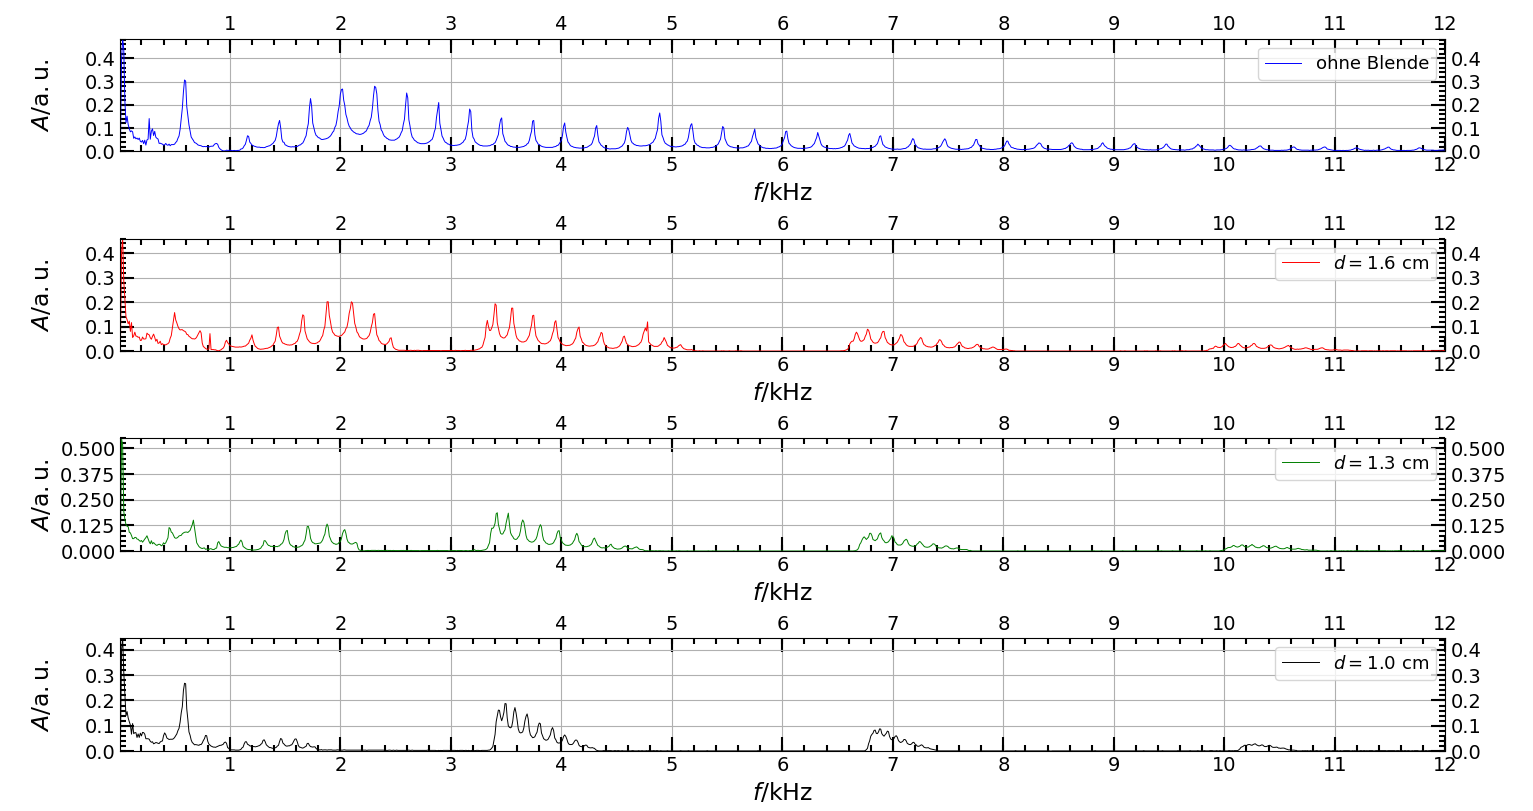
\includegraphics[width=0.9\textwidth]{4612_und_4613.png}
\caption{Spektrum für 11 Irisblenden des Durchmessers $d$}
\end{figure}
\newpage
Es kommt also zur Öffnung von Frequenzbereichen, in denen die Intensität $0$ ist, den Bandlücken. Dementsprechend gibt es auch Frequenzbereiche, in denen sich die Strukturen mit den Peaks befinden. Diese wechseln sich jeweils ab und es ist zu beobachten, dass die Bandlücken umso breiter werden, je kleiner $d$ ist. Dies lässt sich dadurch verstehen, dass für \(d\rightarrow 0\) die Zellen als isoliert betrachtet werden können, d.h. die Kopplung verschwindet dann. Man hat dann den Fall ungekoppelter Atome vorliegen, bei dem sich keine Bandstruktur ausbilden kann. Die Bandstruktur entsteht durch den Überlapp atomarer Wellenfunktionen.
Für 8 bzw. 11 Zylinder der Länge $50$ mm ohne und mit Irisblenden wurde nun jeweils ein Spektrum aufgenommen. Die Resonanzfrequenzen wurden bestimmt und über der zugehörigen Wellenzahl aufgetragen. Dabei sind folgende Aufnahmen entstanden:
\\\\
\begin{figure}[h!]
\centering
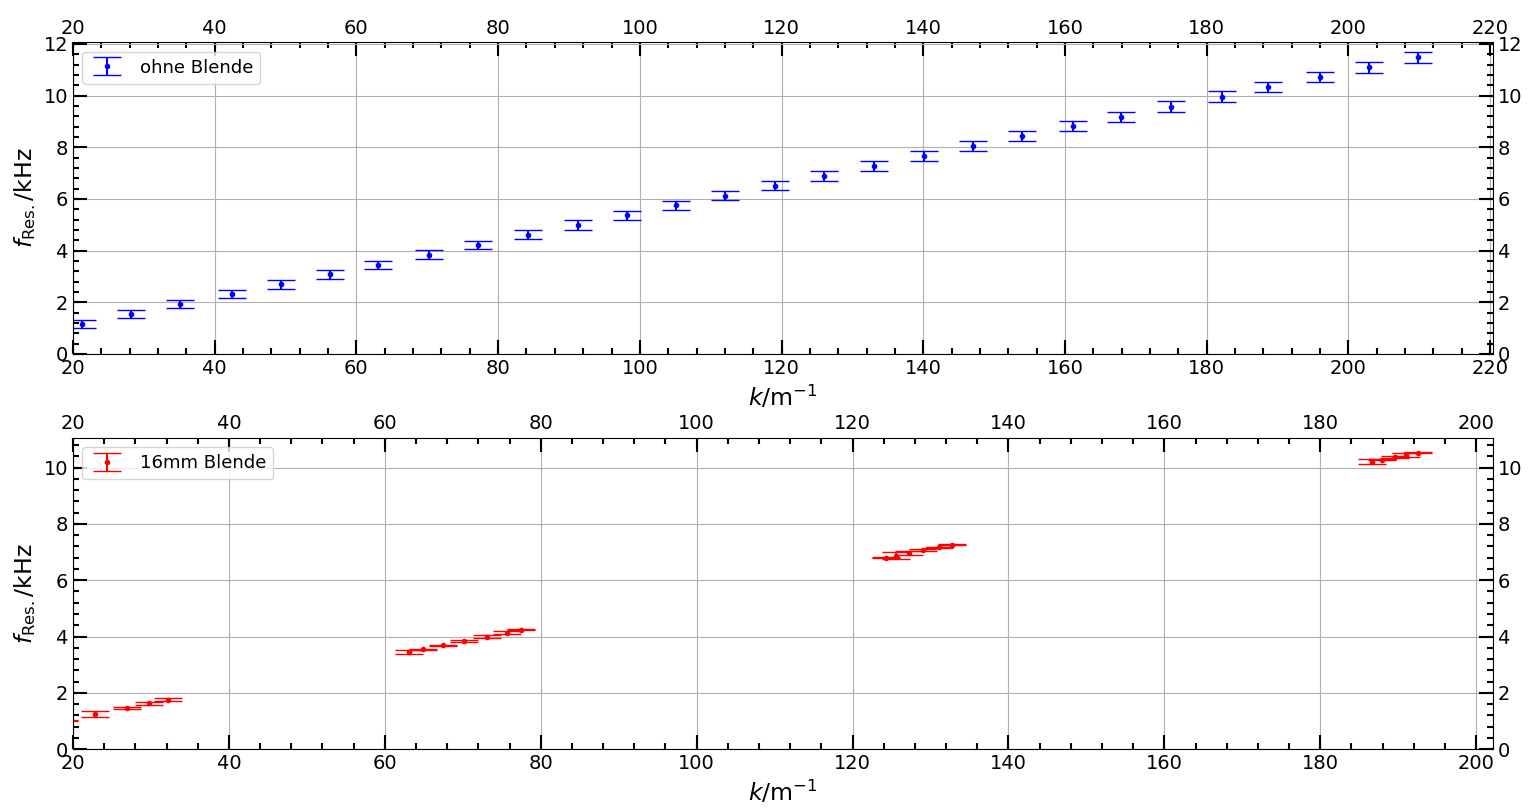
\includegraphics[width=\textwidth]{4614_400mm_mit_und_ohne_Blende.png}
\caption{Resonanzfrequenzen für 8 Zylinder mit und ohne Irisblenden}
\end{figure}
\newpage
\begin{figure}[h!]
\centering
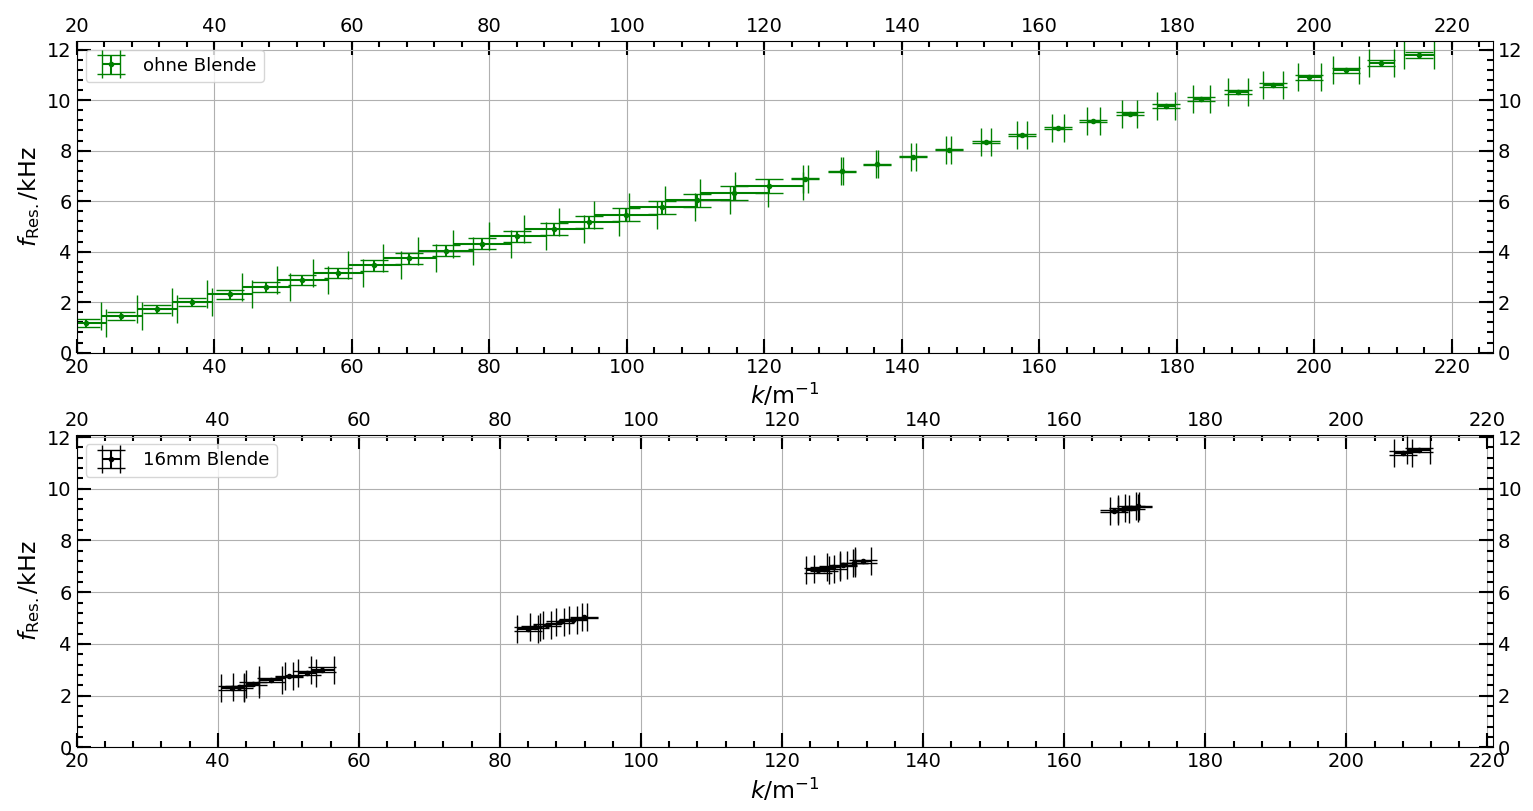
\includegraphics[width=\textwidth]{4615_600mm_mit_und_ohne_Blende.png}
\caption{Resonanzfrequenzen für 11 Zylinder mit und ohne Irisblenden}
\end{figure}
Auch hier ist zu sehen, dass es für den Resonator mit Irisblenden Lücken gibt, in denen keine Resonanzen, also keine Peaks, auftreten. Für die längere Röhre erhält man analog zu den gekoppelten Kugelresonatoren im betrachteten Frequenzbereich mehrere Bänder (Resonanzen) aufgrund der Resonanzbedingung.
\newline Die reduzierten Zonenschemata zu diesen Betrachtungen sind in folgenden Abbildungen gegeben:
\\\\
\begin{figure}[h!]
\centering
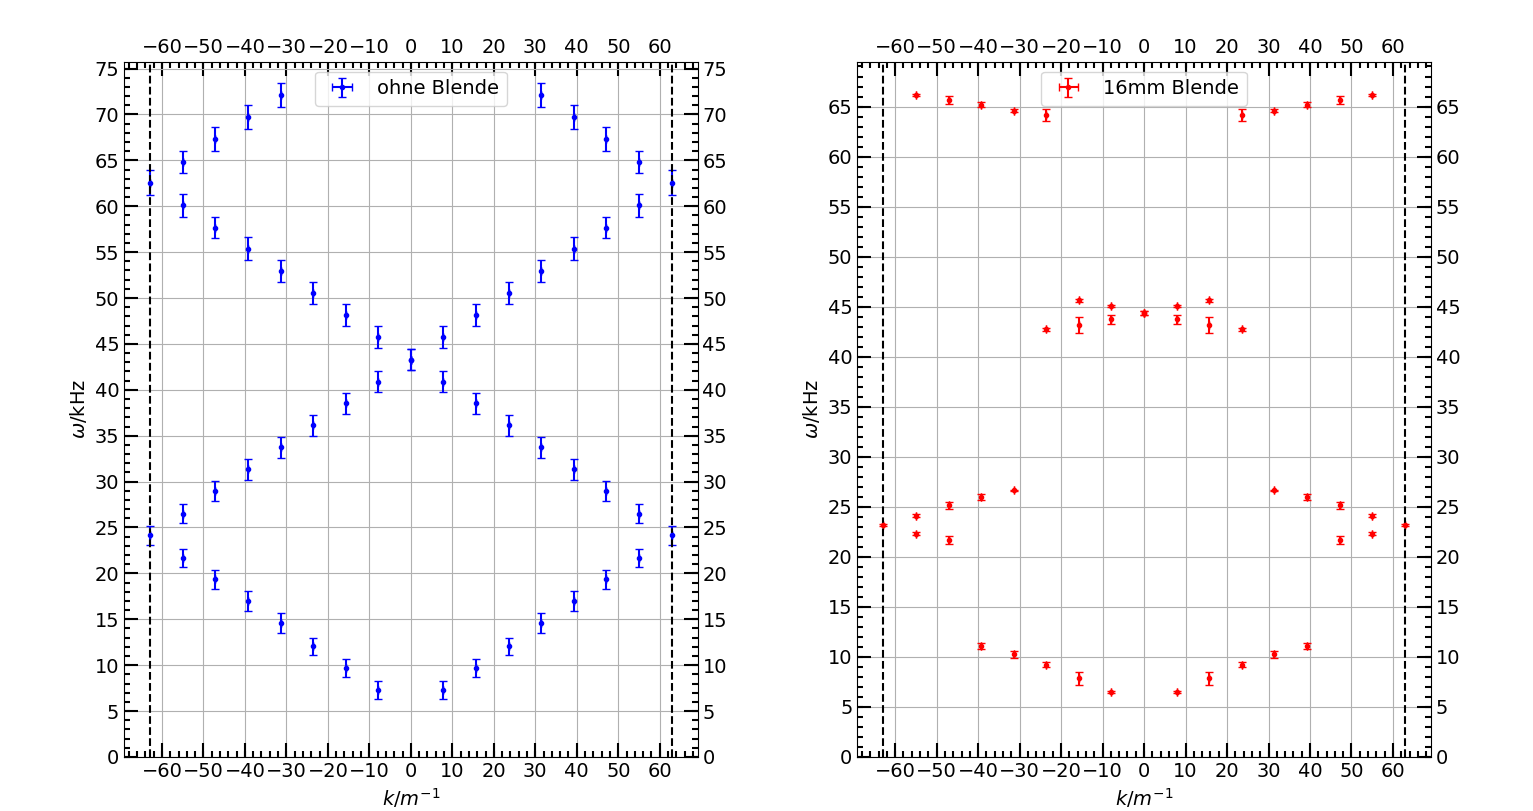
\includegraphics[width=\textwidth]{4614_400mm_reduziertes_Zonenschema.png}
\caption{Reduziertes Zonenschema $L=400$ mm}
\end{figure}
\newpage
\begin{figure}[h!]
\centering
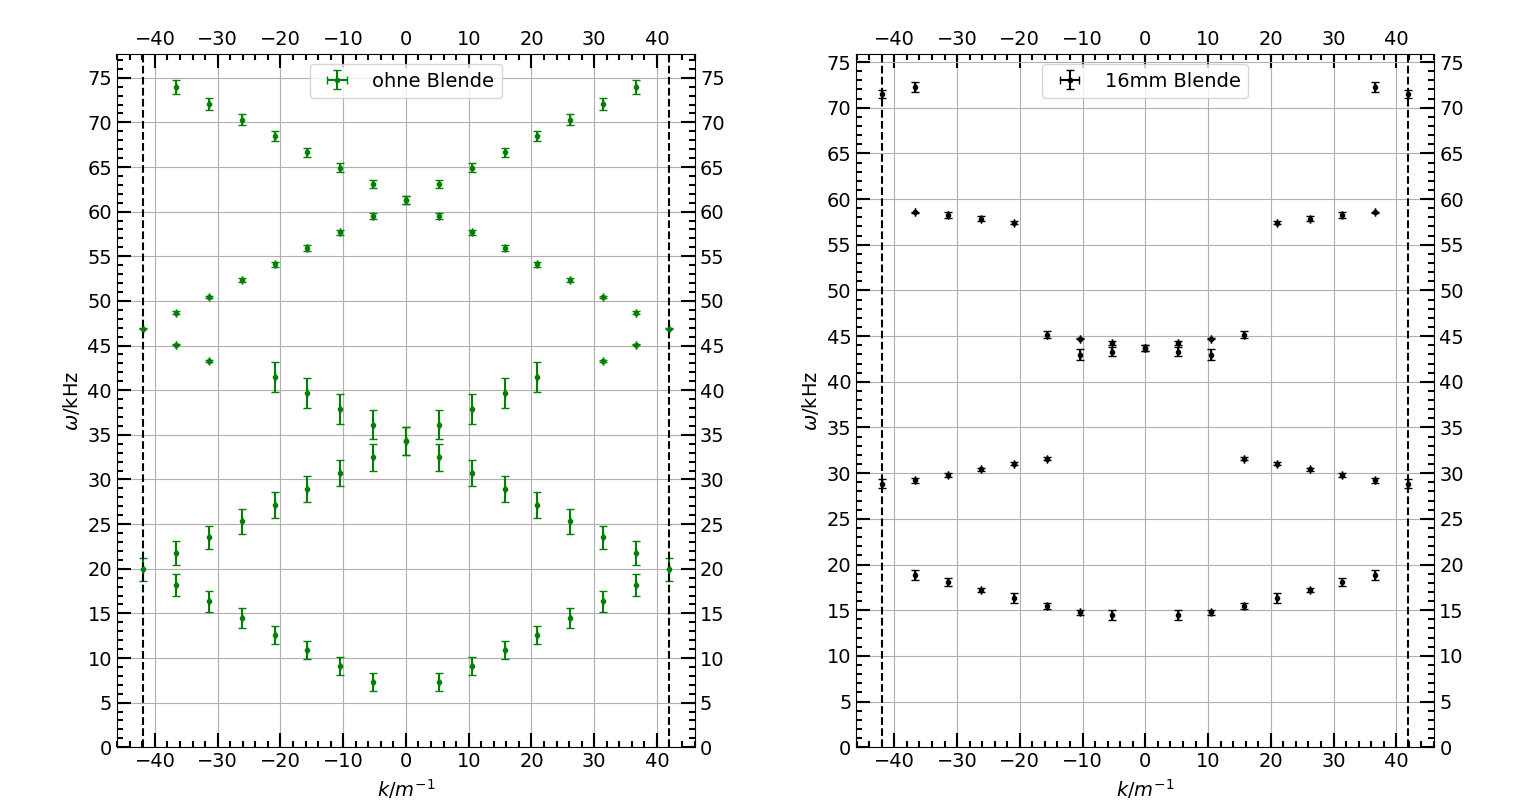
\includegraphics[width=\textwidth]{4615_600mm_reduziertes_Zonenschema.png}
\caption{Reduziertes Zonenschema $L=600$ mm}
\end{figure}
Nun gilt es noch die Abhängigkeit des Spektrums von der Größe der Einheitszellen zu bestimmen. Dazu wurden die $50$ mm Zylinder durch $75$ mm Zylinder ersetzt. Das Resultat ist hier als Plot im Vergleich zu den $50$ mm Zylindern dargestellt:
\\\\
\begin{figure}[h!]
\centering
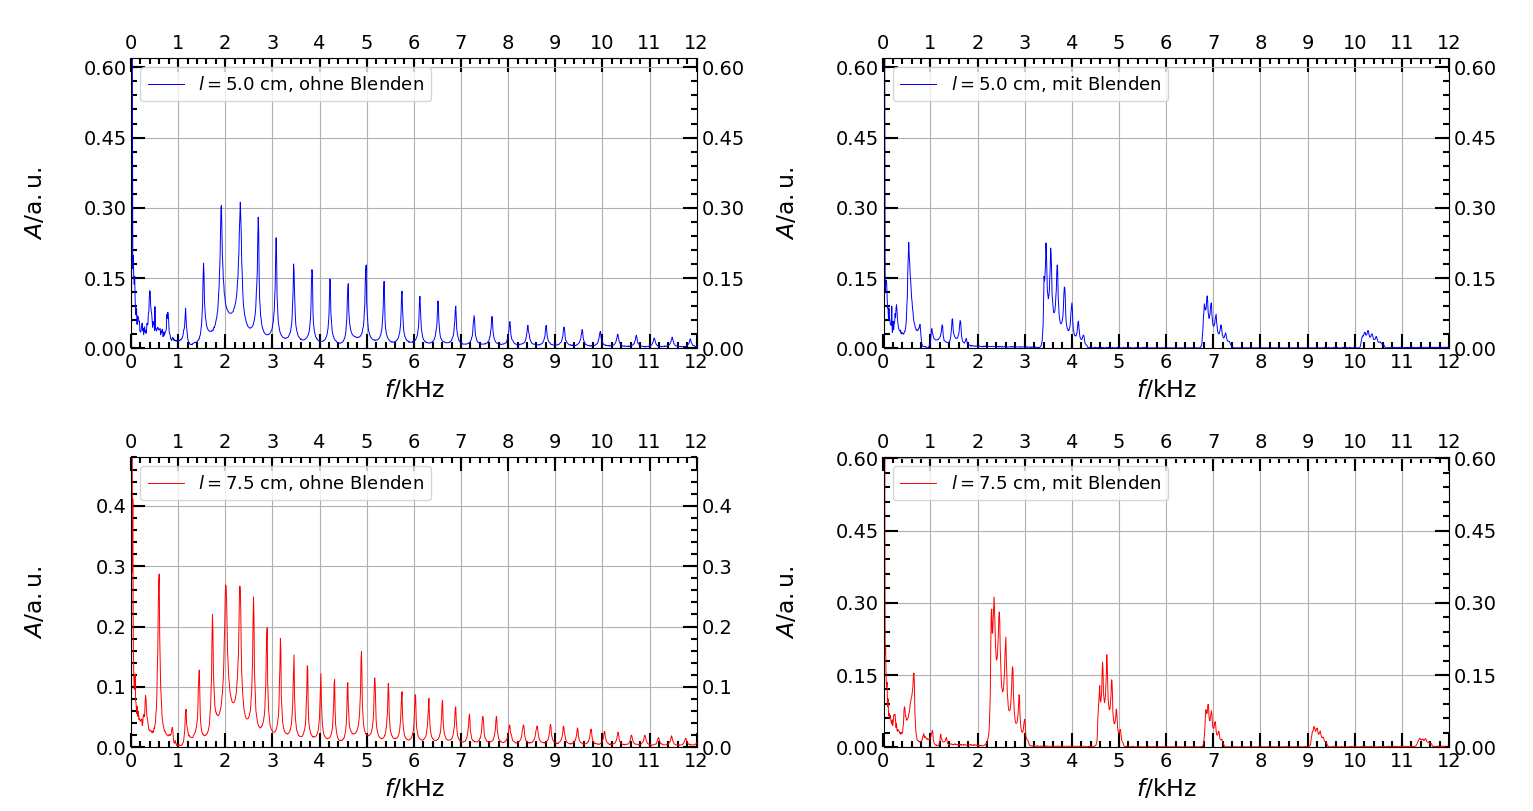
\includegraphics[width=\textwidth]{4614_und_4615.png}
\caption{Spektrum für $50$ mm und $75$ mm Zylinder mit und ohne Blenden}
\end{figure}
\\\\
Für die längeren Zylinder erhält man im selben Frequenzbereich eine größere Anzahl von Bändern. Außerdem haben die Peaks dort eine etwas höhere Intensität. Mit Rückblick auf den Röhrenresonator aus der ersten Teilaufgabe lässt sich das einfach verstehen: Je länger die Zelle, desto kleiner der Modenabstand und desto dichter liegen die Resonanzfrequenzen beieinander.

Schließlich sollte noch die Zustandsdichte für die 8 Zylinder mit je $50$ mm und $16$ mm Irisblenden betrachtet werden. Diese ergibt sich aus dem reziproken Frequenzabstand zu:
\begin{align}
\rho(f)=\frac{1}{f_{i+1}-f_i}
\end{align}
Der zugehörige Plot ist folgender:
\newpage
\begin{figure}[h!]
\centering
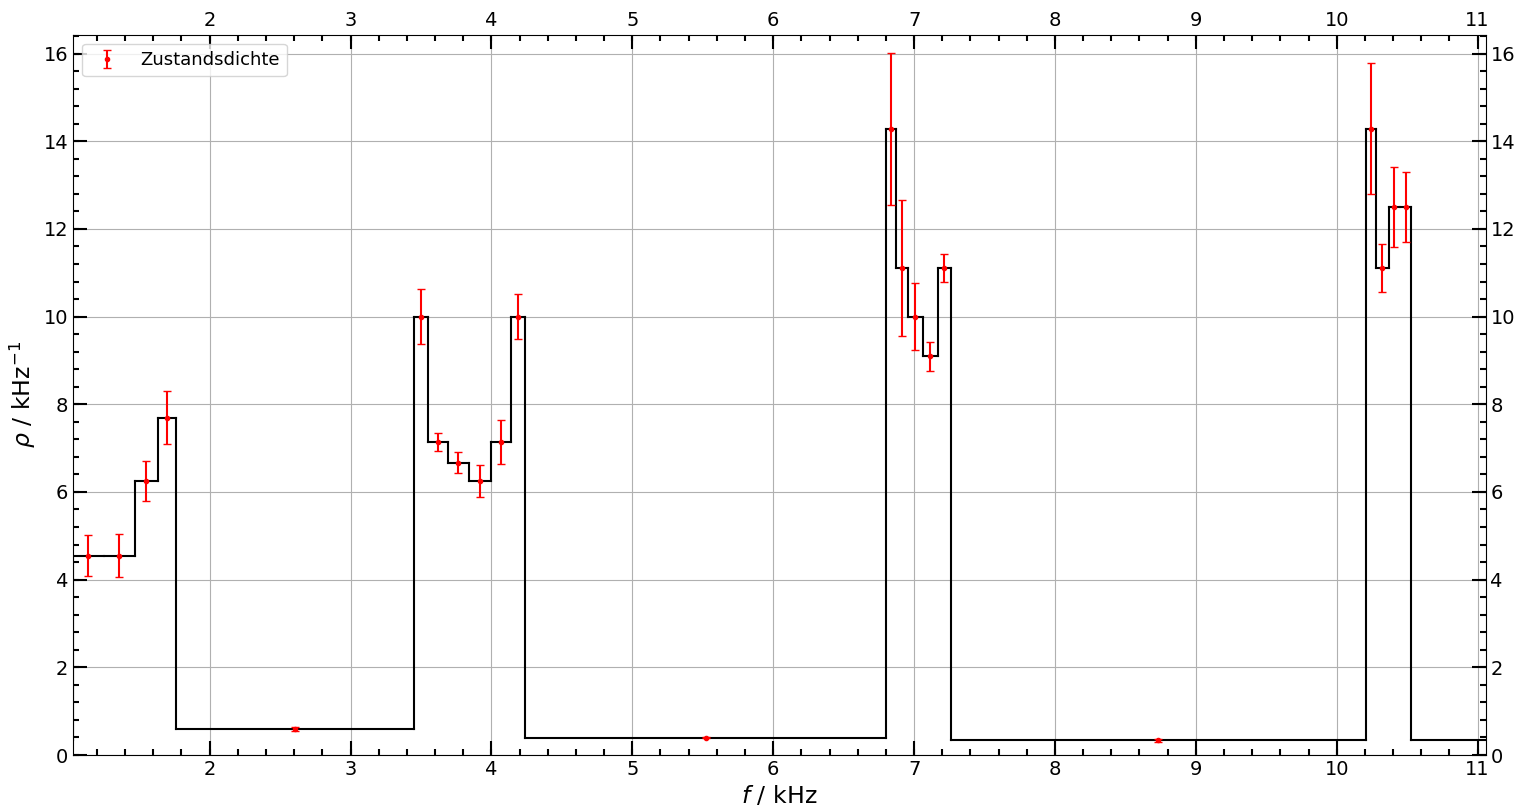
\includegraphics[width=\textwidth]{4614_Zustandsdichte.png}
\caption{Zustandsdichte für 8 Einheitszellen ($50$ mm) mit $16$ mm Blenden}
\end{figure}
Hier sieht man auch nochmals, dass es Bandlücken gibt, in denen keine Resonanzfrequenzen auftreten und somit sind dort auch keine Zustände.
\subsubsection{Atom-Molekül-Kette}
Zuerst sollte das Übersichtsspektrum für einen einzelnen Zylinder der Länge $50$ mm und $75$ mm aufgenommen werden:
\newpage
\begin{figure}[h!]
\centering
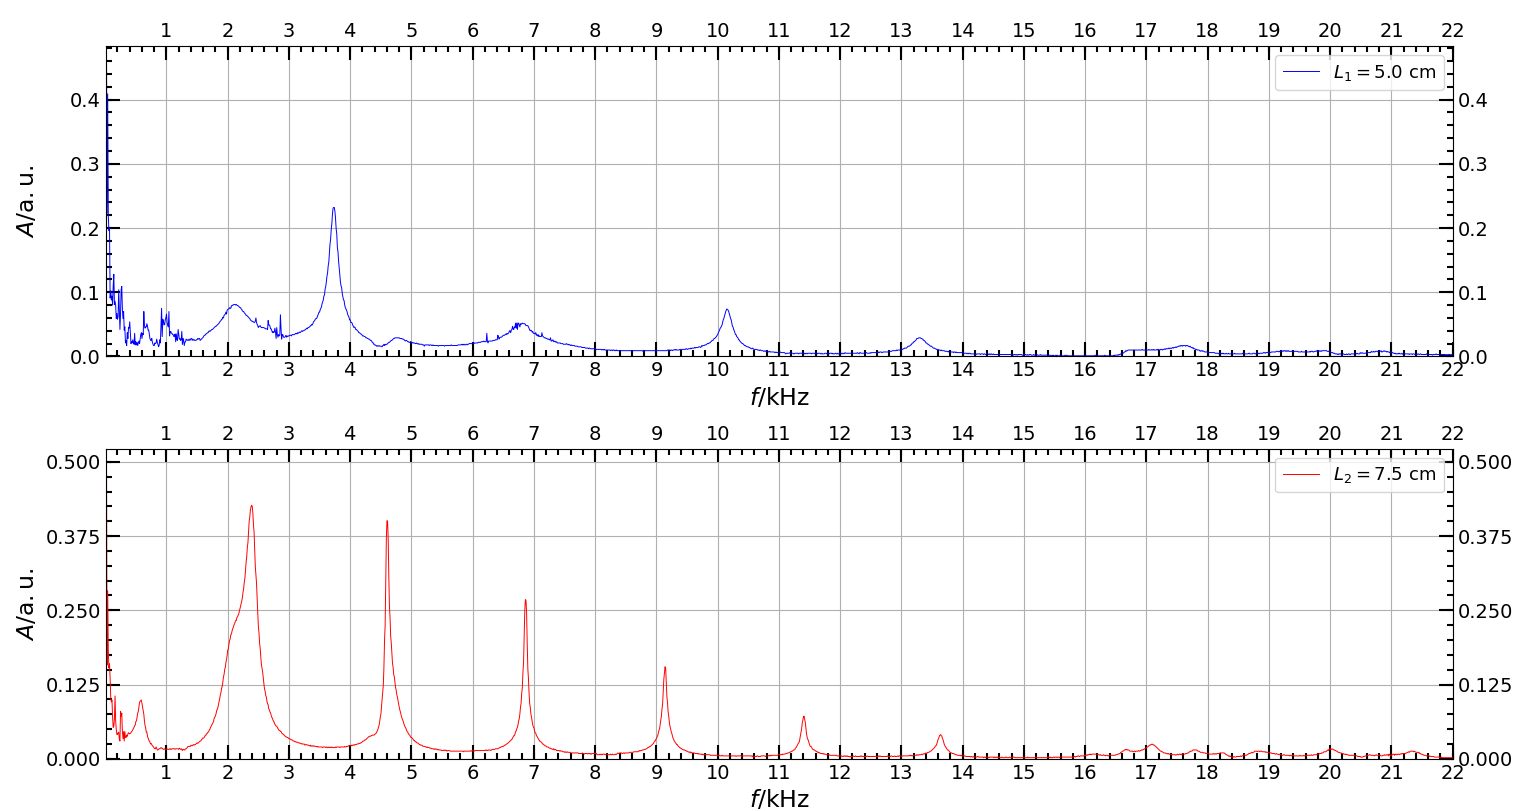
\includegraphics[width=\textwidth]{4621.png}
\caption{Übersichtsspektrum einzelner Zylinder}
\end{figure}
Die longitudinalen Moden (Peaks unter $16$ kHz) sind deutlich ausgeprägter als die radialen Moden (Peaks über $16$ kHz) und für den längeren Zylinder ($75$ mm) haben wir Peaks mit einer höheren Intensität als für $50$ mm. Außerdem sind für den längeren Zylinder mehr Peaks im Frequenzbereich bis $16$ kHz.
Zur Untersuchung der Abhängigkeit des Spektrums vom Irisblendendurchmesser für ein Molekül aus zwei $50$ mm Zylindern wurden folgende Spektren gemessen:
\newpage
\begin{figure}[h!]
\centering
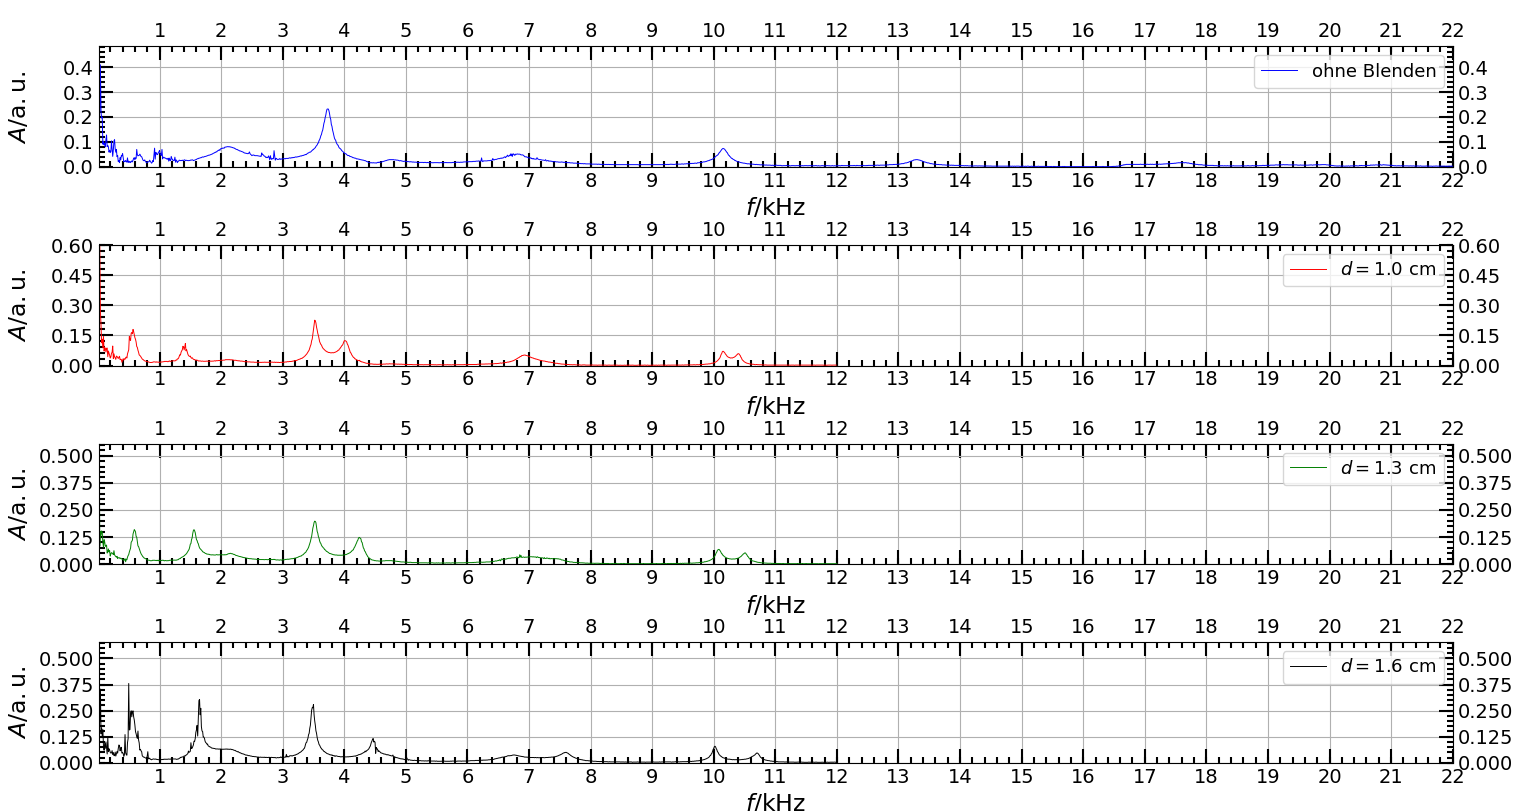
\includegraphics[width=\textwidth]{4622_und_4623.png}
\caption{Spektrum eines Moleküls für verschiedene Irisblenden}
\end{figure}
Mit zunehmendem Blendendurchmesser spalten die Peaks stärker auf. Die Kopplung für die kleinste Irisblende ist dabei schwach, da dies näher am Modell zweier getrennter Atome liegt. Der linke Peak ist jeweils (analog zu den Betrachtungen im Abschnitt zum Molekül) der Bindende.
Um die Entstehung der Bänder mit zunehmender Anzahl an Einheitszellen zu untersuchen, wurde folgende Grafik erstellt:
\begin{figure}[h!]
\centering
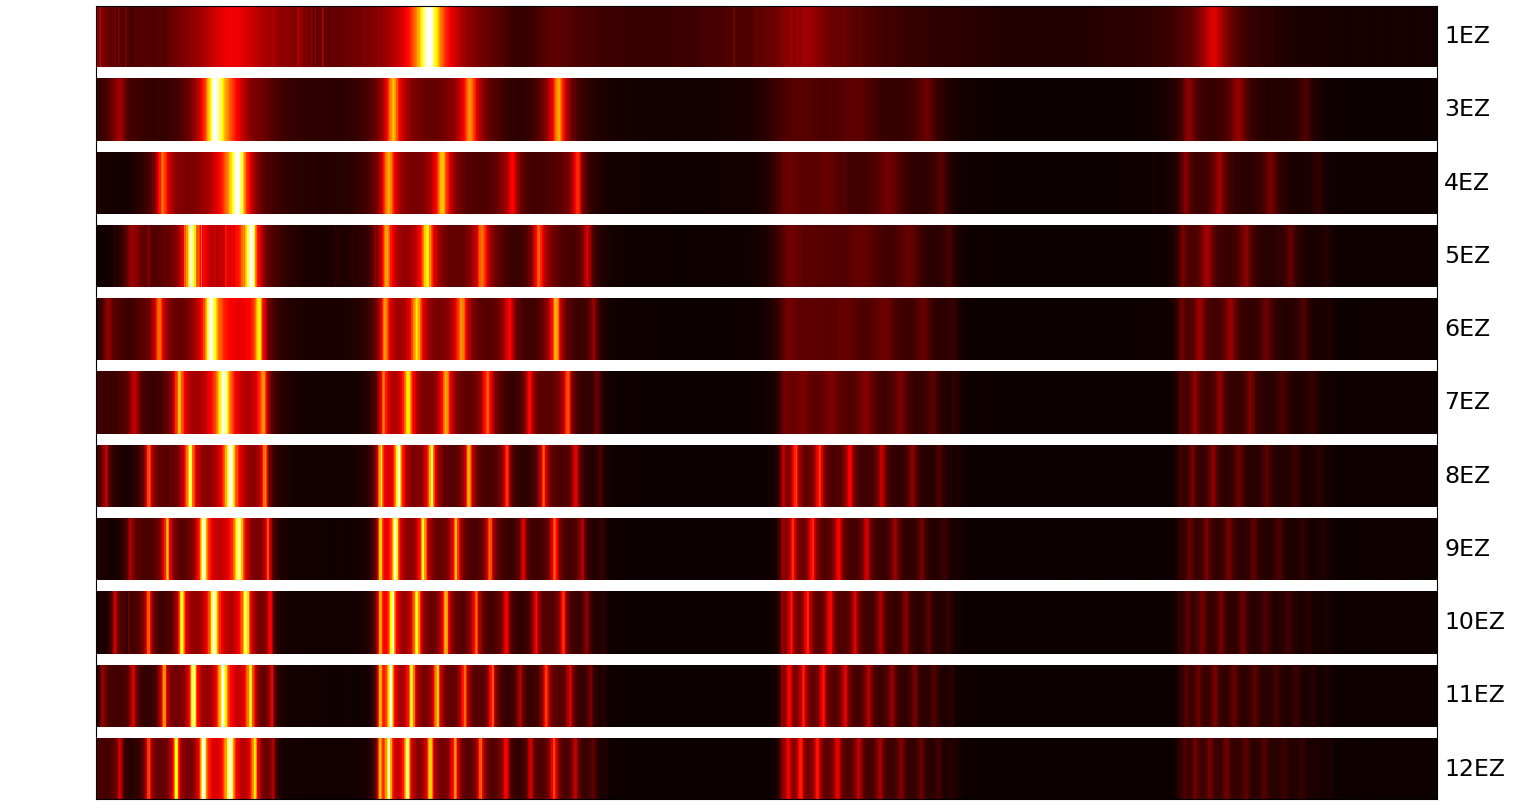
\includegraphics[width=0.9\textwidth]{4624_Entstehung_der_Baender.png}
\caption{Entstehung der Bänder mit steigender Anzahl an Einheitszellen}
\end{figure}
\\\\
Man sieht hier nochmals sehr deutlich, dass jedes Band genauso viele Linien enthält, wie der Festkörper Einheitszellen hat. Ausnahme ist das unterste Band, welches immer genau eine Linie weniger hat. Bei dieser nicht beobachtbaren Linie handelt es sich um die Nullpunktsschwingung. Hierbei ist lediglich zu berücksichtigen, dass die Frequenz immer erst oberhalb von 1 kHz aufgezeichnet wurde, um Messrauschen zu unterdrücken.

\subsubsection{Überstrukturen und Einheitszellen mit mehr als einem Atom}
Für den zu modellierenden Festkörper wurde das Spektrum für $13$ mm Blenden sowie abwechselnd $13$ mm und $16$ mm Blenden aufgenommen:
\\\\
\begin{figure}[h!]
\centering
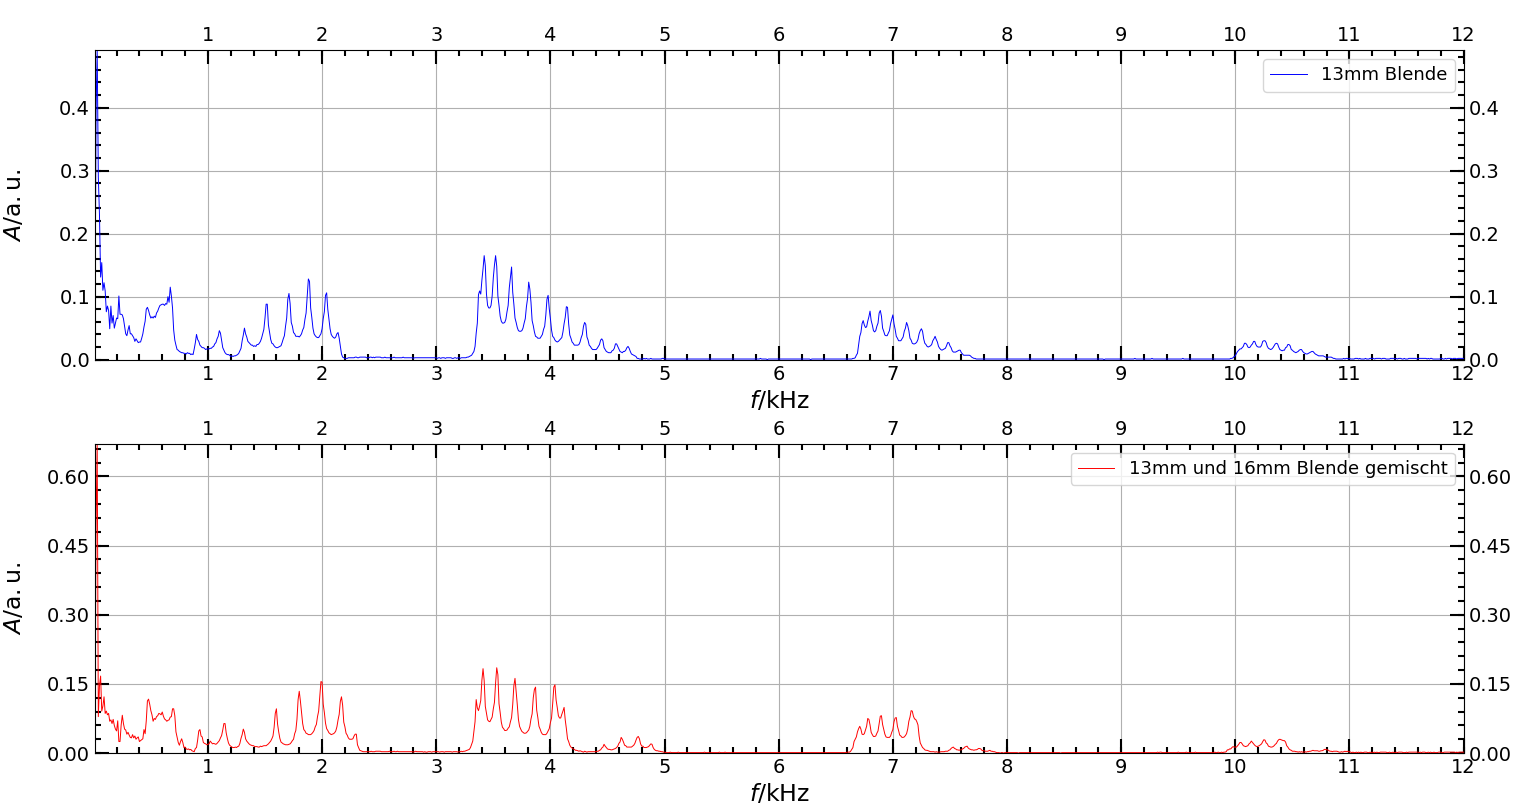
\includegraphics[width=\textwidth]{4631_Uebersichtsspektren.png}
\caption{Übersichtsspektrum $13$ mm Blenden und $13$mm Blenden und $16$ mm Blenden gemischt}
\end{figure}
\\\\
Die für beide Situationen zugehörige Darstellung im reduzierten Zonenschema sieht dann so aus:
\newpage
\begin{figure}[h!]
\centering
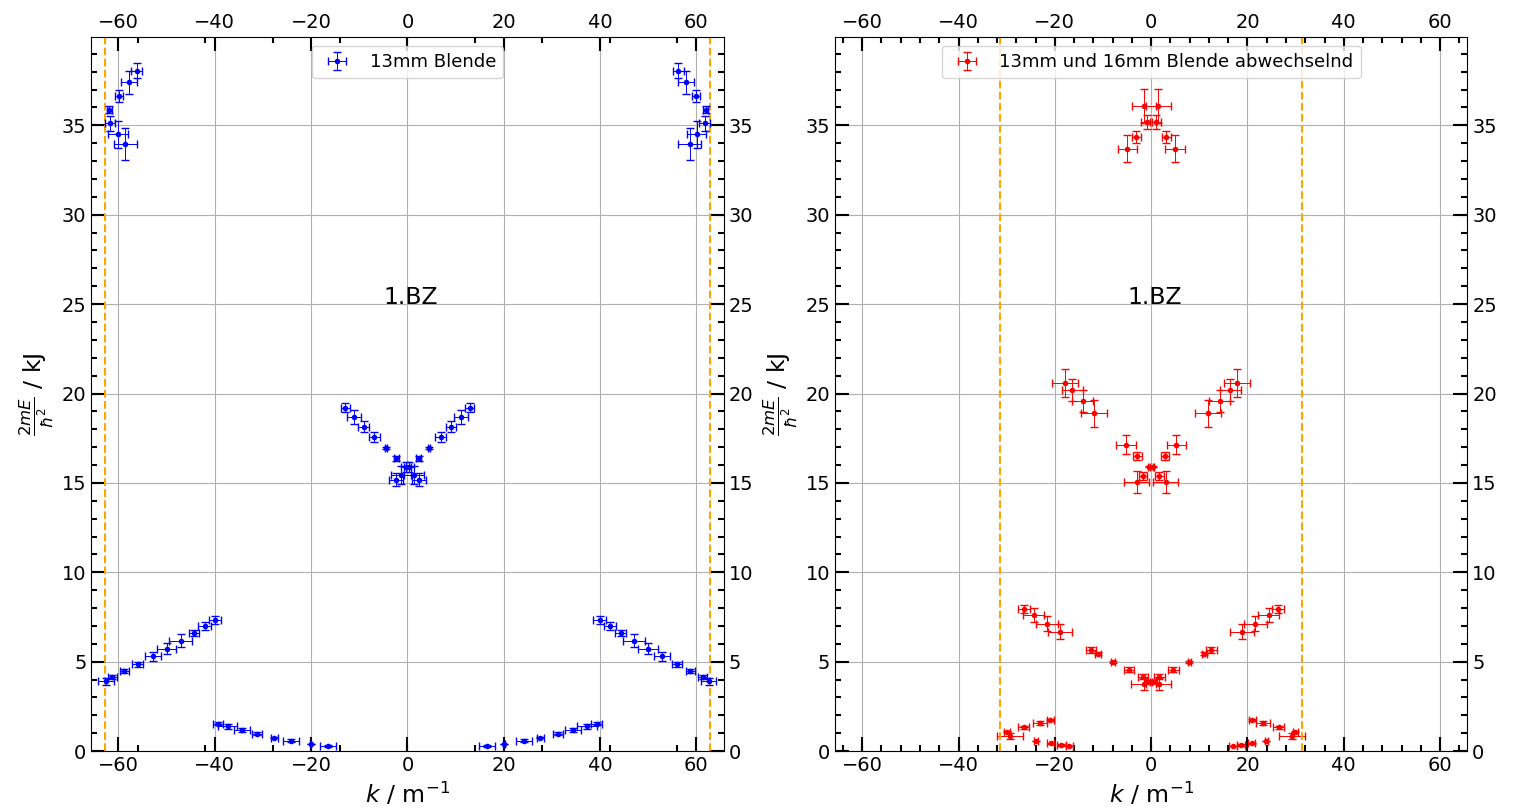
\includegraphics[width=\textwidth]{4631_reduziertes_Zonenschema.png}
\caption{Reduziertes Zonenschema für  $13$ mm Blenden und $13$mm Blenden und $16$ mm Blenden gemischt}
\end{figure}
Auffallend ist, dass im Falle verschieden großer Einheitszellen die Brillouin-Zone wesentlich kleiner wird. Dies liegt daran, dass die Gitterkonstante durch die Überstruktur größer und damit der reziproke Gittervektor kleiner wird. Außerdem treten neben den Bändern neue Strukturen auf; im Spektrum erkennt man diese als kleinere Resonanzen neben den ursprünglichen Bändern. Das lässt sich auf die Störung der Periodizität zurückführen. 
\\\\
Für die Messung des Festkörpers aus 5 Einheitszellen, die jeweils aus $50$mm Zylinder mit einer $16$ mm Irisblende und einem $75$ mm Zylinder mit einer $16$ mm Blende bestehen, ergibt sich folgendes Spektrum und folgendes reduziertes Zonenschema:
\newpage
\begin{figure}[h!]
\centering
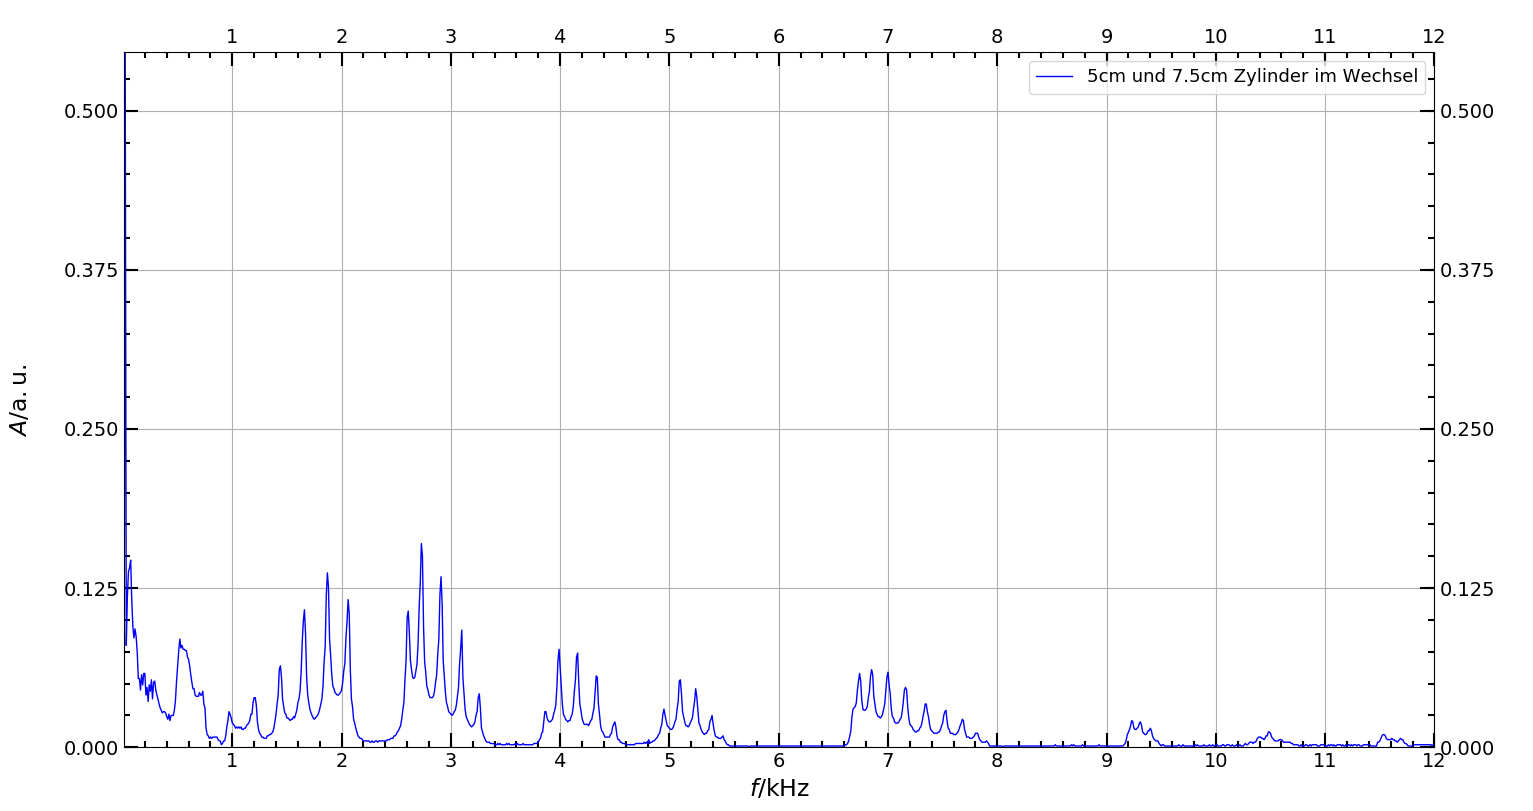
\includegraphics[width=\textwidth]{4632_Uebersichtsspektrum.png}
\caption{Spektrum für 5 Einheitszellen aus $50$mm Zylinder mit einer $16$ mm Irisblende und einem $75$ mm Zylinder mit einer $16$ mm Blende}
\end{figure}
\begin{figure}[h!]
\centering
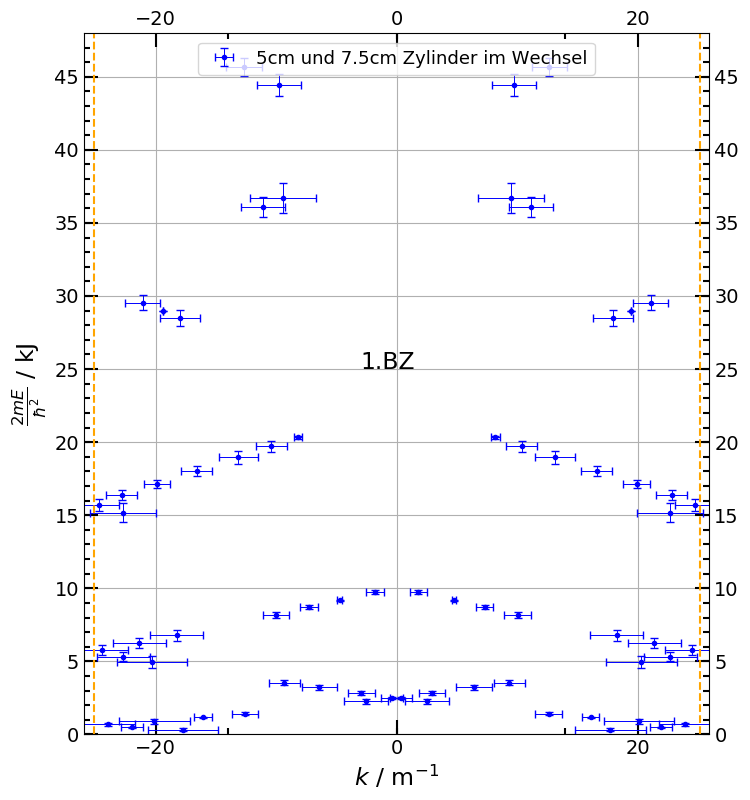
\includegraphics[scale=0.325]{4632_reduziertes_Zonenschema.png}
\caption{Reduziertes Zonenschema für 5 Einheitszellen aus $50$mm Zylinder mit einer $16$ mm Irisblende und einem $75$ mm Zylinder mit einer $16$ mm Blende}
\end{figure}
Um die einzelnen Atome für beide Zylinderlängen miteinander und mit Überstruktur zu vergleichen, werden folgende Abbildungen verwendet:
\begin{figure}[h!]
\centering
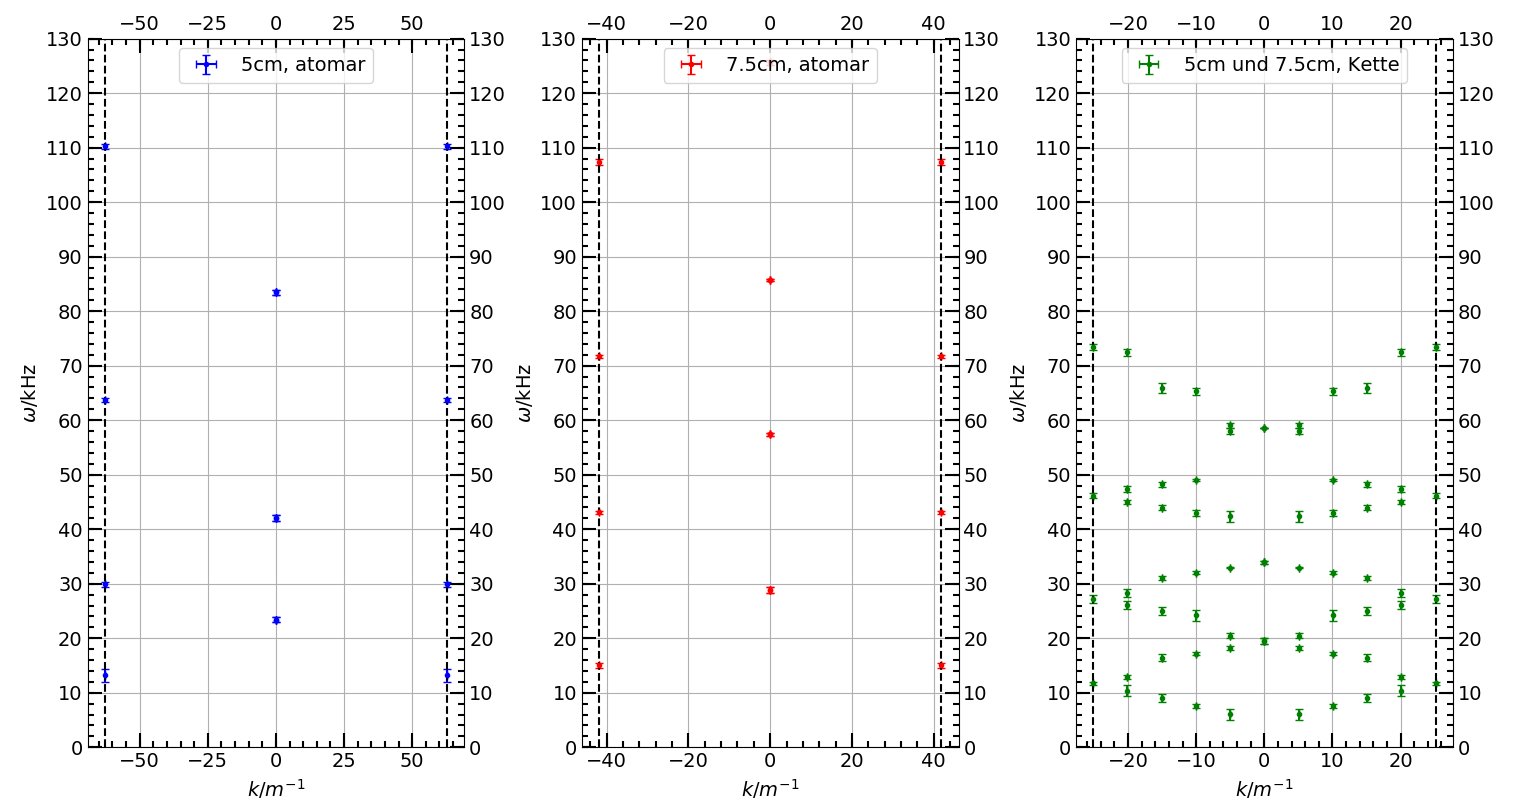
\includegraphics[width=\textwidth]{4632_Vergleich_mit_Atomen.png}
\caption{Vergleich des Zonenschemas der Atome mit der Überstruktur}
\end{figure}
\begin{figure}[h!]
\centering
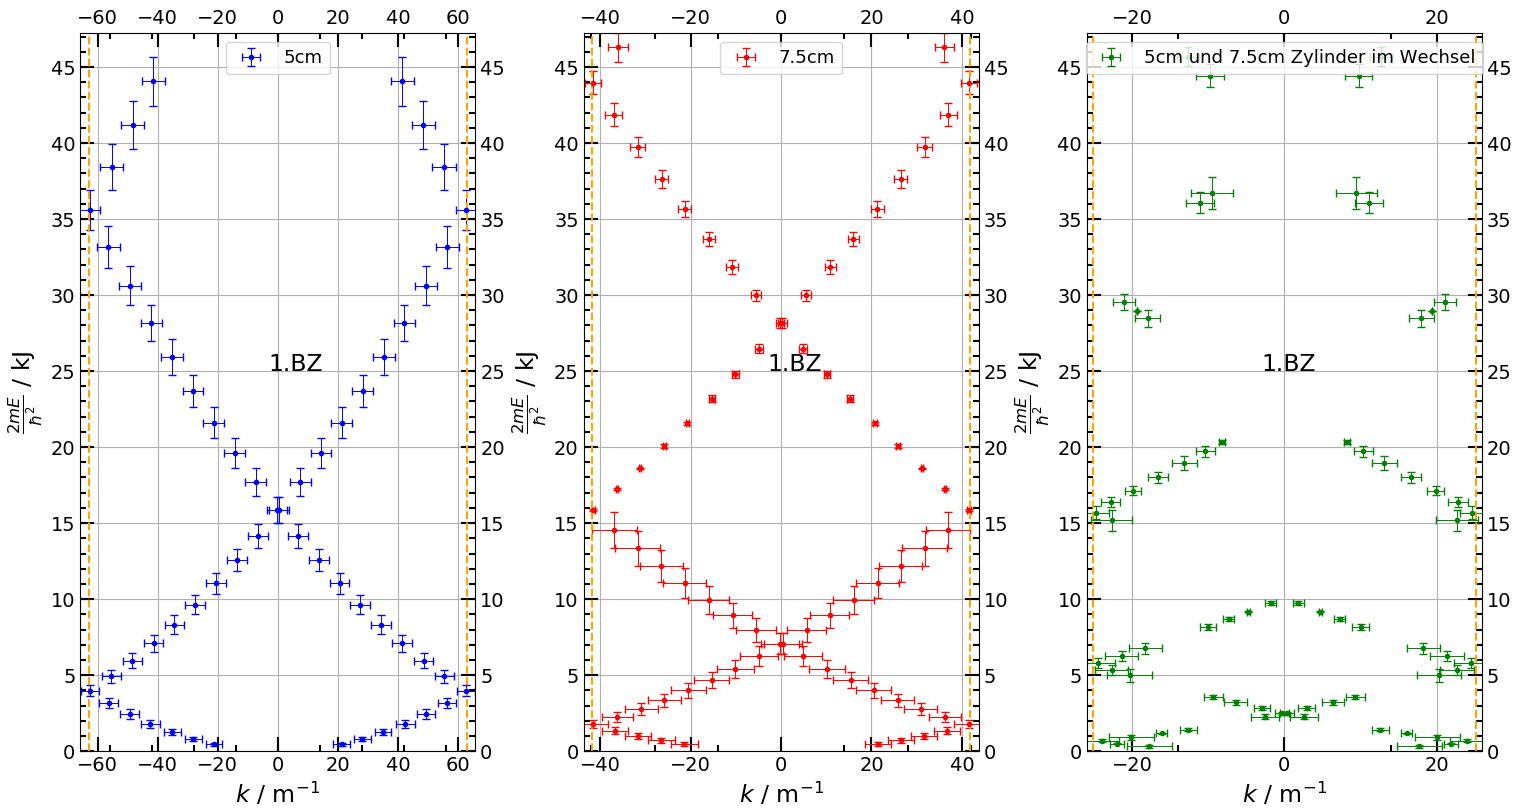
\includegraphics[width=\textwidth]{4632_Vergleich_mit_Atomketten.png}
\caption{Vergleich des Zonenschemas der Atomketten mit der Überstruktur}
\end{figure}
\\\\
Bei Betrachtung und Vergleich der Grafiken könnte man annehmen, dass die Zustände für die einzelnen Atome bei Zusammenfügen derer zu einer Überstruktur miteinander gemischt werden. Aus dieser Mischung der Zustände entsteht dann die Grafik der Überstruktur.
\\\\
Als eigene Kombination für eine Überstruktur wurde ein Festkörper aufgebaut mit 2 $75$ mm Zylindern und einem $50$ mm Zylinder, die jeweils durch eine $16$ mm Blende getrennt sind. Dies ergab folgendes reduziertes Zonenschema:
\\\\
\begin{figure}[h!]
\centering
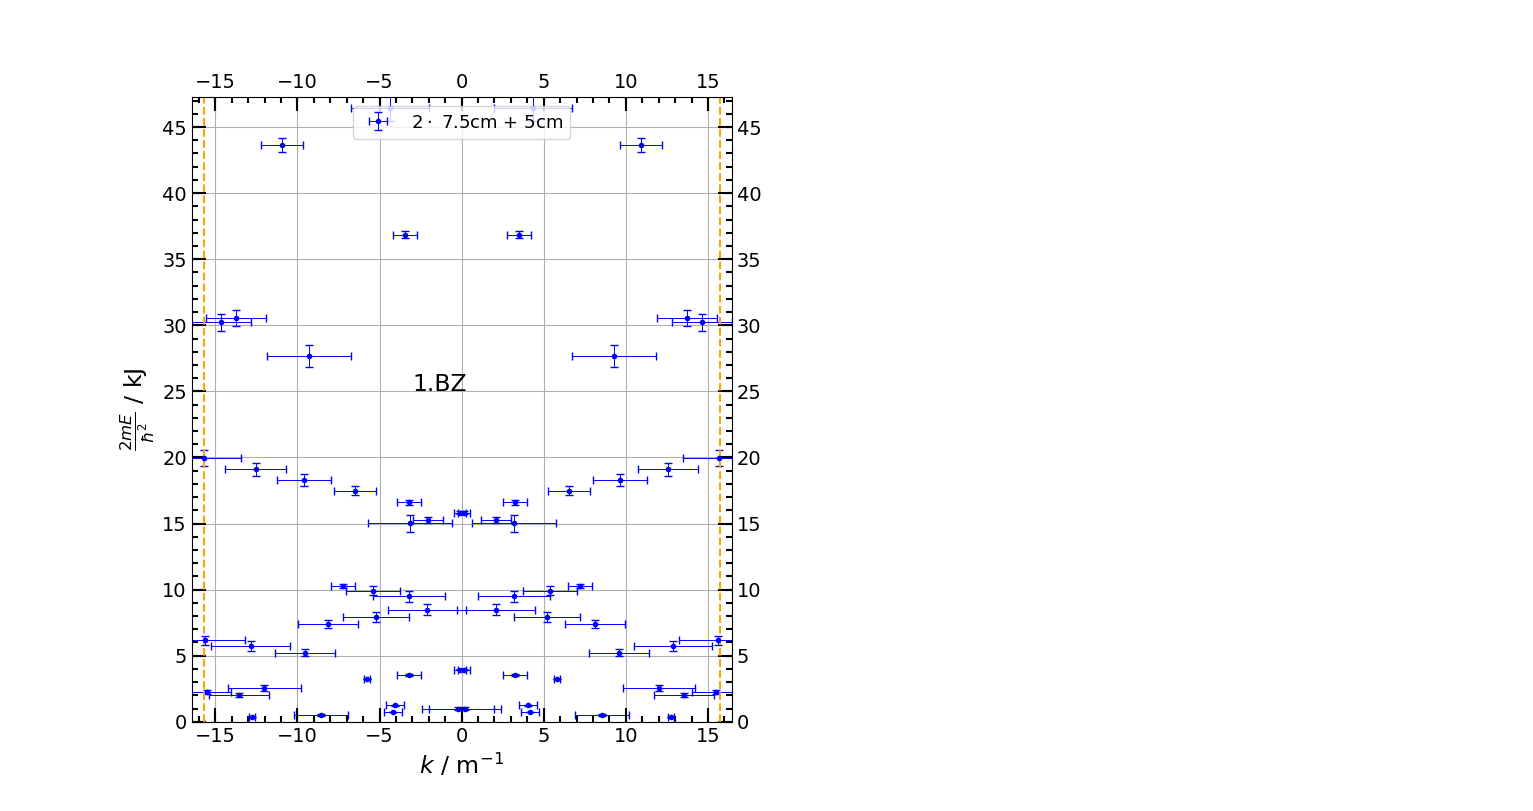
\includegraphics[width=\textwidth]{4633_reduziertes_Zonenschema.png}
\caption{Reduziertes Zonenschema für eigene Überstruktur}
\end{figure}
\\\\
Die Brioullin-Zone wird nochmals ersichtlich kleiner, weil die Periodizität länger geworden ist. Außerdem verschieben sich die Zustände neu, sodass man sehr viele Zustände niedriger Energie und auffallend große Bandlücken in den höheren Niveaus hat. 

\subsubsection{Defekte}
Um eine Störung zu simulieren, wird ein Festkörper aus 12 $50$ mm Zylindern mit $16$ mm Blenden aufgebaut und dann ein Zylinder durch einen $75$ mm Zylinder ersetzt. Der Defekt wurde einmal an 6. und einmal an 9. Stelle eingebaut. Die Spektren sahen dann so aus:
\\\\
\begin{figure}[h!]
\centering
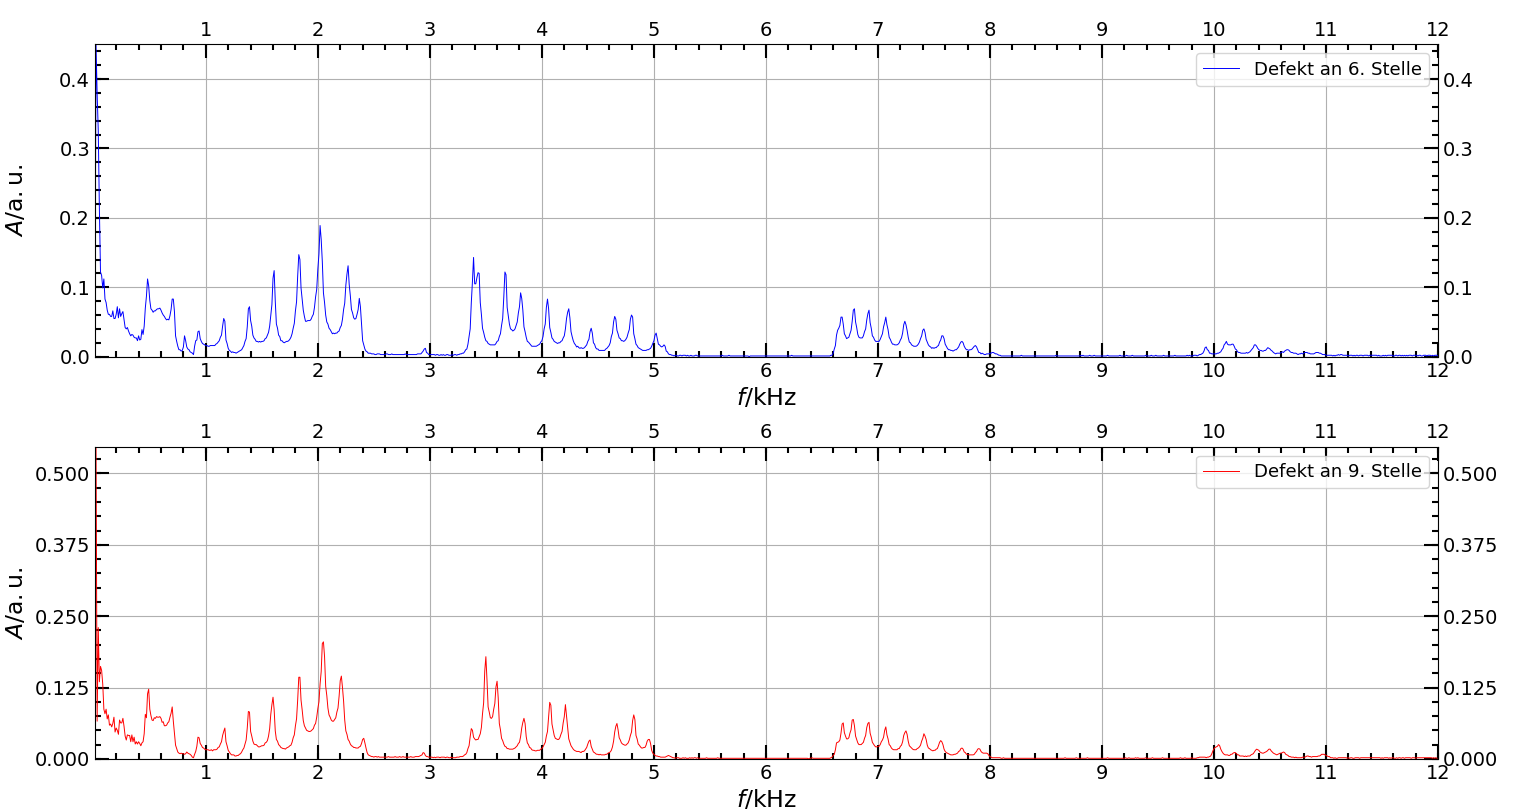
\includegraphics[width=\textwidth]{4641_und_4642_Uebersichtssprektren.png}
\caption{Übersichtsspektren für Defekt an 6. bzw. an 9. Stelle}
\end{figure}
\\\\
Die zugehörigen reduzierten Zonenschemata sind diese:
\\\\
\begin{figure}[h!]
\centering
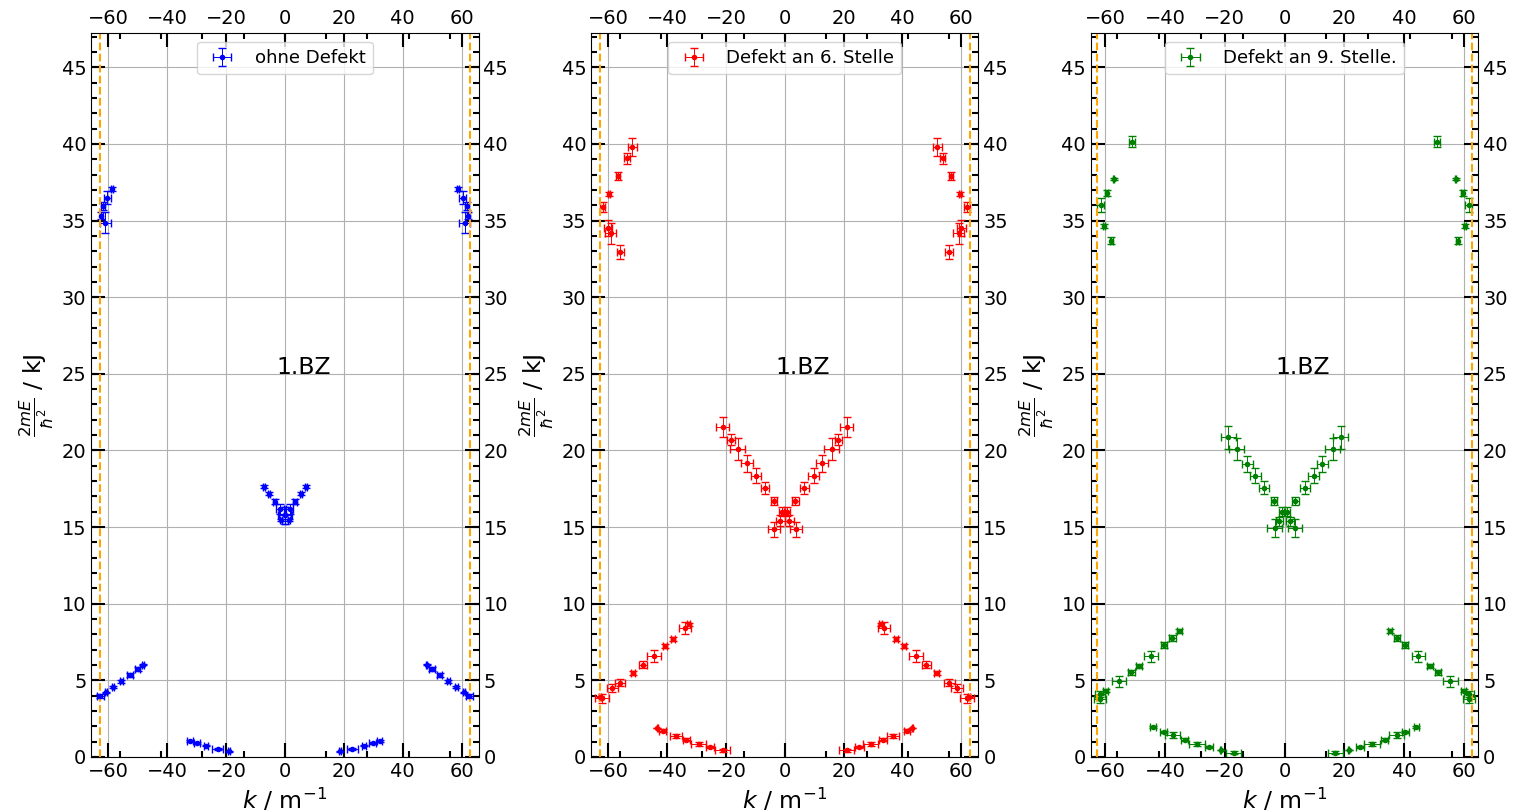
\includegraphics[width=\textwidth]{4641_und_4642_reduziertes_Zonenschema.png}
\caption{Reduzierte Zonenschemata für Defekt an 6. bzw. an 9. Stelle}
\end{figure}
Insbesondere im reduzierten Zonenschema lässt sich deutlich erkennen, dass die genaue Position des Defektes im Rahmen der Messgenauigkeit keinen wesentlichen Einfluss auf die Eigenschaften des Festkörpers hat. Dies kommt der realen Situation im Festkörper nahe. Was eine Rolle spielen könnte wäre die Anzahl der Defekte sowie deren Verteilung (stark lokalisiert oder gut verteilt). Gleichzeitig ist aber auch erkennbar, dass sich das Zonenschema mit Defekt deutlich von dem ohne Defekt unterscheidet. Der Defekt erzeugt zusätzliche Niveaus und beeinflusst damit wesentlich die Eigenschaften des Festkörpers (vgl. Dotierung von Halbleitern).
\section{Fazit}
Der Versuch trägt sehr zum Verständnis quantenmechanischer Effekte in Atomen, Molekülen und Festkörpern bei. Jedoch ist dabei stets zu beachten, dass lediglich ein qualitativer und kein quantitativer Vergleich stattfinden kann. \\\\
Außerdem gibt es Phänomene die rein-quantenmechanischer Natur sind und daher durch diesen Versuch gar nicht nachgebildet werden können, etwa die Nullpunktsschwingung. An solchen Stellen sollte man sich trotz aller Analogie stets den fundamentalen Unterschied zwischen klassischer Betrachtung und Quantenmechanik bewusst machen. \\\\
Darüber hinaus konnte die Schallgeschwindigkeit durch Resonanzphänomene bestimmt werden. Die Erzeugung und Vermessung von Resonanzen stellt eine wichtige Technik dar, durch die Frequenzen zu den besonders genau bestimmbaren Größen gehören.


    % Bibliographie/Literaturverzeichnis
    \begin{thebibliography}{9}
    \bibitem{Anleitung}
    Versuchsanleitung Quantenanalogie, Fortgeschrittenenpraktikum Physik TU Dresden
    \end{thebibliography}
% Ende Dokument

\end{document}
